% !TEX program = pdflatex
\documentclass[12pt,a4paper]{report}

% ---------- Packages ----------
\usepackage[utf8]{inputenc}
\usepackage[T1]{fontenc}
\usepackage{lmodern}
\usepackage[french]{babel}
\usepackage[a4paper,margin=2cm]{geometry}
\usepackage{graphicx}
\usepackage[table]{xcolor}
\usepackage{array}
\usepackage{booktabs}
\usepackage{longtable}
\usepackage{tabularx}
\usepackage{enumitem}
\usepackage{fancyhdr}
\usepackage{listings}
\usepackage{float}
\usepackage{amsmath,amssymb}
\setlength{\headheight}{15pt}
\usepackage[hidelinks,pdftitle={EasyVote - Rapport de Test},pdfauthor={Talel Mejri, Rawen Zgarni, Issra Elakrout},pdfsubject={Ingenierie des Tests et Validations}]{hyperref}

\definecolor{evblue}{HTML}{4F46E5}
\definecolor{evlight}{HTML}{E0E7FF}
\definecolor{codebg}{HTML}{F5F5F5}
\definecolor{okgreen}{HTML}{15803D}
\definecolor{kored}{HTML}{B91C1C}
\definecolor{paorange}{HTML}{B45309}
\definecolor{negray}{HTML}{6B7280}

\setlist{itemsep=2pt,topsep=4pt}
\setlength{\parindent}{0pt}
\setlength{\parskip}{6pt}

% ---------- Header / footer ----------
\pagestyle{fancy}
\fancyhf{}
\fancyhead[L]{EasyVote --- Rapport de Test}
\fancyhead[R]{\thepage}
\fancyfoot[C]{\footnotesize\color{negray}T. Mejri \textbullet\ R. Zgarni \textbullet\ I. Elakrout \quad|\quad 2026--2027}
\renewcommand{\headrulewidth}{0.4pt}
\renewcommand{\footrulewidth}{0pt}
\fancypagestyle{plain}{\fancyhf{}\fancyhead[L]{EasyVote --- Rapport de Test}\fancyhead[R]{\thepage}\fancyfoot[C]{\footnotesize\color{negray}T. Mejri \textbullet\ R. Zgarni \textbullet\ I. Elakrout \quad|\quad 2026--2027}\renewcommand{\headrulewidth}{0.4pt}\renewcommand{\footrulewidth}{0pt}}

% ---------- Code listing ----------
\lstset{
  basicstyle=\ttfamily\footnotesize,
  backgroundcolor=\color{codebg},
  frame=single,
  breaklines=true,
  columns=fullflexible,
  keepspaces=true,
  showstringspaces=false,
  literate={é}{{\'e}}1 {è}{{\`e}}1 {à}{{\`a}}1 {ê}{{\^e}}1 {ç}{{\c c}}1 {ô}{{\^o}}1
           {É}{{\'E}}1 {î}{{\^i}}1 {û}{{\^u}}1 {ù}{{\`u}}1 {â}{{\^a}}1 {’}{{'}}1
           {«}{{\guillemotleft}}1 {»}{{\guillemotright}}1
}

% ---------- Macros ----------
% Statut d'exécution d'un cas de test
\newcommand{\ok}{\textcolor{okgreen}{\textbf{Réussi}}}
\newcommand{\ko}{\textcolor{kored}{\textbf{Échec}}}
\newcommand{\pa}{\textcolor{paorange}{\textbf{Partiel}}}
\newcommand{\nex}{\textcolor{negray}{Non exécuté}}
\newcommand{\aex}{\textcolor{paorange}{À exécuter}}

% Établissement : à renseigner pour l'afficher sur la page de garde (laisser vide sinon)
\newcommand*{\etablissement}{}

\newcommand{\planHead}{\rowcolor{evlight}\textbf{Réf.} & \textbf{Type} & \textbf{Scénario} & \textbf{Prio.} & \textbf{Données} & \textbf{Résultat attendu} & \textbf{Résultat}}

% ======================================================
\begin{document}

% ---------- Page de garde ----------
\begin{titlepage}
\thispagestyle{empty}
\centering

\noindent\colorbox{evblue}{\parbox{\dimexpr\textwidth-2\fboxsep\relax}{\centering\vspace{0.35cm}%
  {\color{white}\large\bfseries INGÉNIERIE DES TESTS ET VALIDATIONS\par}%
  \vspace{3pt}{\color{white}\small Rapport de projet --- Qualité logicielle\par}\vspace{0.35cm}}}

\vspace{1.2cm}
\ifx\etablissement\empty\else{\large\bfseries\etablissement\par}\vspace{1cm}\fi

{\Huge\bfseries Rapport de Test\par}
\vspace{0.5cm}
{\color{evblue}\rule{0.4\textwidth}{1.5pt}\par}
\vspace{0.7cm}
{\fontsize{46}{54}\selectfont\bfseries\color{evblue} EasyVote\par}
\vspace{0.3cm}
{\Large Plateforme Web de Vote Universitaire\par}
\vspace{0.6cm}
{\large\itshape Plan de test, gestion des tests avec Testiny, exécution du plan\\
et organisation du travail d'équipe avec Jira\par}

\vspace{1.6cm}
\fcolorbox{evblue}{evlight}{\begin{minipage}{\dimexpr\textwidth-2\fboxsep-2\fboxrule\relax}
\vspace{0.35cm}
\begin{minipage}[t]{0.47\linewidth}
\raggedright
\textbf{\color{evblue}Réalisé par}\\[5pt]
Talel Mejri\\
Rawen Zgarni\\
Issra Elakrout
\end{minipage}\hfill
\begin{minipage}[t]{0.47\linewidth}
\raggedright
\textbf{\color{evblue}Module}\\[5pt]
Ingénierie des Tests et Validations\\[8pt]
\textbf{\color{evblue}Enseignant}\\[5pt]
Dr. Ing. Faouzi Jaidi
\end{minipage}
\vspace{0.35cm}
\end{minipage}}

\vfill
{\color{evblue}\rule{\textwidth}{0.6pt}\par}
\vspace{4pt}
{\large Octobre 2026\par}
{\large Année universitaire 2026--2027\par}
\end{titlepage}

\pagenumbering{roman}
\chapter*{Résumé}
\addcontentsline{toc}{chapter}{Résumé}

\textbf{EasyVote} est une plateforme web de vote universitaire dont l'exigence centrale est l'\textbf{anonymat cryptographique} du scrutin. Ce rapport décrit la démarche de test de l'équipe : expression de 15 exigences traçables, plan de 68 cas de test sur quatre niveaux (unitaire, intégration, système, acceptation), puis exécution avec des techniques statiques et dynamiques, manuelles et automatisées. Le travail d'équipe est organisé avec \textbf{Jira} (méthode Scrum) et les tests sont gérés dans \textbf{Testiny}.

\begin{table}[H]
\centering
\caption{Chiffres clés de l'exécution}
\small
\begin{tabularx}{\textwidth}{@{}p{6.4cm}X@{}}
\toprule
\rowcolor{evlight}\textbf{Indicateur} & \textbf{Valeur}\\
\midrule
Exigences identifiées & 15\\
Cas de test du plan & 68\\
Tests JUnit automatisés & 38 : 36 réussis, 2 en échec (défauts détectés)\\
Scénario de démonstration de bout en bout & 12 vérifications sur 12 réussies\\
Défauts détectés & 9 : 1 critique, 5 majeurs, 3 mineurs\\
Couverture de code (JaCoCo) & 100\,\% des branches de la génération des jetons ; 38,0\,\% des lignes du projet\\
\bottomrule
\end{tabularx}
\end{table}

\textbf{Conclusion principale.} Le scénario de démonstration fonctionne, mais l'\textbf{anonymat du vote n'est pas garanti} : une jointure SQL permet de relier un électeur à son vote (DEF-00, défaut critique). Sa correction est la priorité absolue, suivie des défauts de sécurité DEF-05 et DEF-06.

\clearpage
\tableofcontents
\clearpage
\listoftables
\listoffigures
\clearpage

\chapter*{Abréviations}
\addcontentsline{toc}{chapter}{Abréviations}
\begin{tabularx}{\textwidth}{@{}p{2.6cm}X@{}}
\toprule
\rowcolor{evlight}\textbf{Sigle} & \textbf{Signification}\\
\midrule
CDC & Cahier des charges\\
EX-xx & Exigence identifiée\\
DEF-xx & Défaut détecté\\
UT, IT, ST, UAT & Tests unitaire, d'intégration, système, d'acceptation (\textit{User Acceptance Test})\\
REG, ...-Mxx & Test de régression (ou de maintenance)\\
MC/DC & \textit{Modified Condition/Decision Coverage}\\
V(G) & Complexité cyclomatique\\
JWT & \textit{JSON Web Token}\\
OTP & \textit{One-Time Password}, code à usage unique\\
RBAC & \textit{Role-Based Access Control}, contrôle d'accès par rôle\\
SaaS & \textit{Software as a Service}\\
\bottomrule
\end{tabularx}
\clearpage
\pagenumbering{arabic}

% ======================================================
\chapter*{Introduction}
\addcontentsline{toc}{chapter}{Introduction}

Ce rapport présente le travail de test réalisé sur la plateforme \textbf{EasyVote}, application web de vote universitaire destinée aux étudiants, aux candidats et à l'administration. Il répond, dans l'ordre, aux cinq objectifs suivants :

\begin{table}[H]
\centering
\caption{Objectifs du travail de test et organisation du rapport}
\small
\begin{tabularx}{\textwidth}{@{}p{0.6cm}Xp{4.2cm}@{}}
\toprule
\rowcolor{evlight}\textbf{N°} & \textbf{Objectif} & \textbf{Où dans ce rapport}\\
\midrule
1 & Choisir le projet & Chapitre~\ref{ch:projet}\\
2 & Présenter les besoins fonctionnels et non fonctionnels & Chapitre~\ref{ch:besoins}\\
3 & Utiliser un outil de gestion des tests et des exigences & Chapitre~\ref{ch:outil} (Testiny)\\
4 & Élaborer un plan de test (niveaux et types) & Chapitre~\ref{ch:plan}\\
5 & Exécuter le plan (techniques statiques et dynamiques, tests manuels et automatisés) & Chapitre~\ref{ch:execution}\\
\bottomrule
\end{tabularx}
\end{table}

Une attention particulière est portée à l'\textbf{anonymat cryptographique du vote}, exigence centrale et différenciante du projet. L'exécution a d'ailleurs révélé que cette exigence n'est pas respectée par le code actuel (défaut critique DEF-00, section~\ref{sec:anonymat}).

Le travail a été réparti entre les trois membres de l'équipe avec \textbf{Jira} (chapitre~\ref{ch:jira}), tandis que \textbf{Testiny} (chapitre~\ref{ch:outil}) gère les cas de test, les exécutions et leurs résultats.

% ======================================================
\chapter{Choix et Présentation du Projet}\label{ch:projet}

\section{Identité du Projet}
EasyVote est une plateforme web de vote universitaire qui digitalise l'intégralité du processus électoral : phase de campagne (présentation des candidats et engagement avec les électeurs), phase de vote (scrutin sécurisé et anonyme) et phase post-électorale (publication des résultats). La plateforme s'appuie sur \textbf{Spring Boot 3.3.5 (Java 21)}, \textbf{React + TypeScript} et \textbf{MySQL/MariaDB}, et intègre un assistant virtuel hybride (règles + IA optionnelle) ainsi qu'un centre de notifications.

\section{Contexte et Objectifs}
Les élections étudiantes reposent encore largement sur des processus traditionnels (bulletins papier, urnes physiques, dépouillement manuel), ce qui entraîne une faible participation (35--40\,\%), une lourdeur organisationnelle (10 à 15 jours de préparation) et un manque de transparence. Le projet poursuit cinq objectifs principaux :
\begin{enumerate}
  \item Digitaliser le processus électoral de bout en bout.
  \item Garantir l'anonymat et l'intégrité du vote grâce à une architecture cryptographique séparant l'identité de l'électeur de son bulletin.
  \item Augmenter la participation électorale par une expérience moderne, accessible depuis tout appareil.
  \item Favoriser l'engagement civique (likes, commentaires, questions/réponses, annonces).
  \item Démontrer la maîtrise des principes du génie logiciel (architecture en couches, sécurité, tests, documentation).
\end{enumerate}

\section{Pourquoi EasyVote comme support de test}
EasyVote est un bon support de test car il réunit des exigences variées et vérifiables :
\begin{itemize}
  \item des \textbf{règles métier précises} (cycle de vie d'une élection, vote unique, limites de saisie), idéales pour les techniques boîte noire ;
  \item un \textbf{cœur algorithmique} (jetons SHA-256, méthode de vote) adapté aux techniques boîte blanche ;
  \item des \textbf{exigences non fonctionnelles} mesurables (temps de réponse, sécurité JWT, contrôle d'accès) ;
  \item une exigence \textbf{critique} (anonymat) dont l'échec aurait un impact majeur, ce qui justifie une approche de test basée sur les risques.
\end{itemize}

\section{Parties Prenantes}
\begin{table}[H]
\centering
\caption{Parties prenantes du projet EasyVote}
\small
\begin{tabularx}{\textwidth}{@{}p{3cm}p{3.2cm}X@{}}
\toprule
\rowcolor{evlight}\textbf{Acteur} & \textbf{Rôle} & \textbf{Responsabilités}\\
\midrule
Étudiants (\texttt{STUDENT}) & Public principal & Consulter les élections, voter, liker, commenter, poser des questions, postuler comme candidat\\
Candidats (\texttt{CANDIDATE}) & Acteurs de campagne & Gérer leur programme, publier des annonces, répondre aux questions, consulter les statistiques d'engagement\\
Administrateur (\texttt{ADMIN}) & Superviseur & Créer/gérer les élections, valider les candidatures, générer les jetons, suivre les statistiques temps réel (ne vote pas)\\
\bottomrule
\end{tabularx}
\end{table}

\section{Code Source du Projet}
Le code source (backend Spring Boot, frontend React, scripts de configuration et de seed) ainsi que tous les tests réalisés (dossiers \texttt{easyvote-backend/src/test} et \texttt{tests/}) sont versionnés sur le dépôt :
\url{https://github.com/LtayefAhmed/EasyVote}

% ======================================================
\chapter{Organisation du Travail d'Équipe avec Jira}\label{ch:jira}

\section{Pourquoi un outil de gestion de projet}
Le projet est réalisé par trois personnes qui travaillent en parallèle sur le code, les tests et le rapport. Sans outil commun, le risque est de dupliquer un travail, d'oublier un test ou de ne plus savoir qui fait quoi. L'équipe a donc adopté \textbf{Jira}, outil de gestion de projet agile, avec la méthode \textbf{Scrum} : un backlog de tâches priorisées, un sprint de durée fixe et un tableau d'avancement partagé.

\section{Mise en place du projet Jira}
\begin{itemize}
  \item Un espace \textbf{Easy Vote} de type Scrum, partagé par les trois membres : Talel Mejri (TM), Rawen Zgarni (RZ) et Issra Elakrout (IE). Chaque ticket est assigné à un membre.
  \item \textbf{Cinq epics}, un par famille de tests : boîte noire, boîte blanche, unitaires, intégration et acceptation.
  \item Des \textbf{tâches}, une par test automatisé (38 au total), et des \textbf{bugs} pour les défauts DEF-xx trouvés pendant l'exécution.
  \item Un backlog \textbf{importé en une seule fois} depuis le fichier \texttt{tests/backlog-jira.csv}, généré à partir de la liste des tests du script \texttt{lancer-tests.ps1}. Chaque ticket reprend l'identifiant du plan (PE-01, R1, IT-04\ldots), la classe et la méthode JUnit, la commande de lancement et le résultat attendu : un ticket Jira correspond directement à un test exécutable.
  \item Un \textbf{workflow} à quatre états : \textit{To Do}, \textit{In Progress}, \textit{In Review}, \textit{Done}. L'état \textit{In Review} prévoit la relecture du travail par un autre membre avant la clôture, ce qui correspond à la revue entre pairs du cours (section~\ref{sec:statique-cours}).
  \item Une \textbf{priorité} (de \textit{Highest} à \textit{Low}) fixée selon le risque métier, comme dans la stratégie du chapitre~\ref{ch:plan}, et des \textbf{étiquettes} indiquant le type et le niveau du test.
\end{itemize}

\paragraph{Définition du « terminé ».} Un ticket passe en \textit{Done} lorsque le test est écrit, exécuté (\texttt{lancer-tests.ps1 <identifiant>}), son résultat consigné et le travail relu par un autre membre.

\section{Sprint 1 : backlog et tableau}
Le \textbf{sprint 1} (du 1\textsuperscript{er} au 8 octobre) regroupe 11 tickets de l'epic « Tests boîte noire ». La figure~\ref{fig:jira-backlog} montre le backlog du sprint (référence, résumé, epic, statut, priorité, responsable) et la figure~\ref{fig:jira-tableau} le tableau Scrum. Au moment de la capture, 5 tickets sont terminés (\textit{Done}), 4 sont en relecture (\textit{In Review}), 1 est en cours et 1 reste à faire.

\begin{figure}[H]
\centering
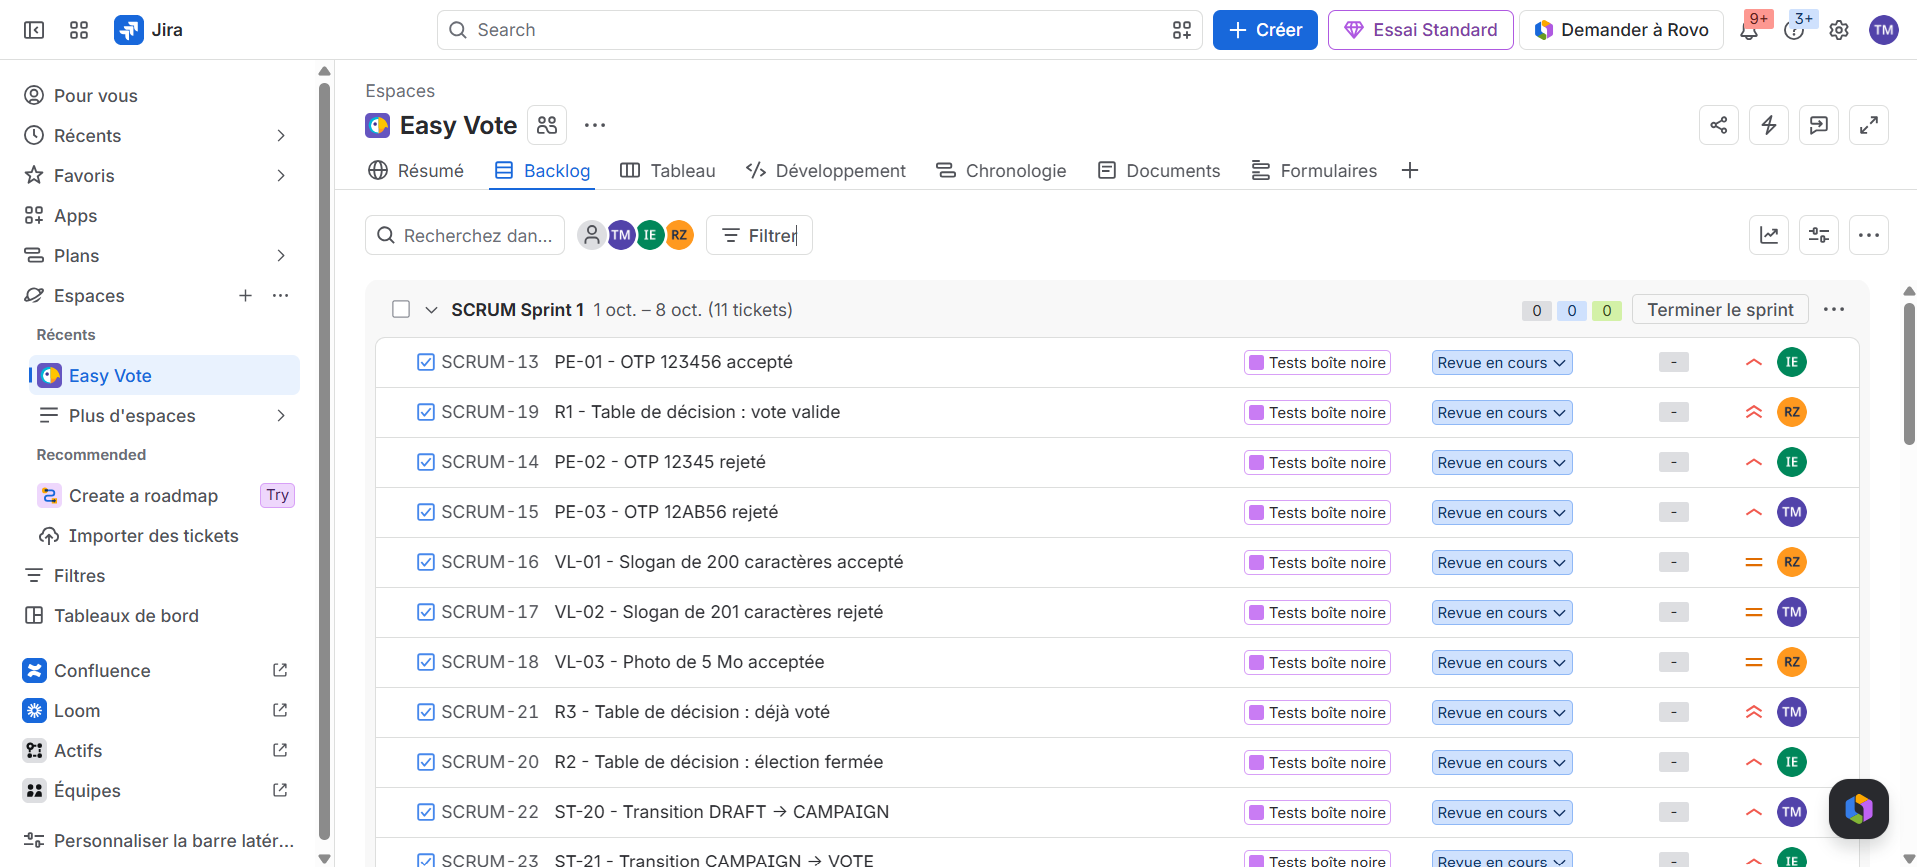
\includegraphics[width=\textwidth]{images/jira-backlog.png}
\caption{Jira --- backlog du sprint 1 : tickets de l'epic « Tests boîte noire », avec statut, priorité et responsable}\label{fig:jira-backlog}
\end{figure}

\begin{figure}[H]
\centering
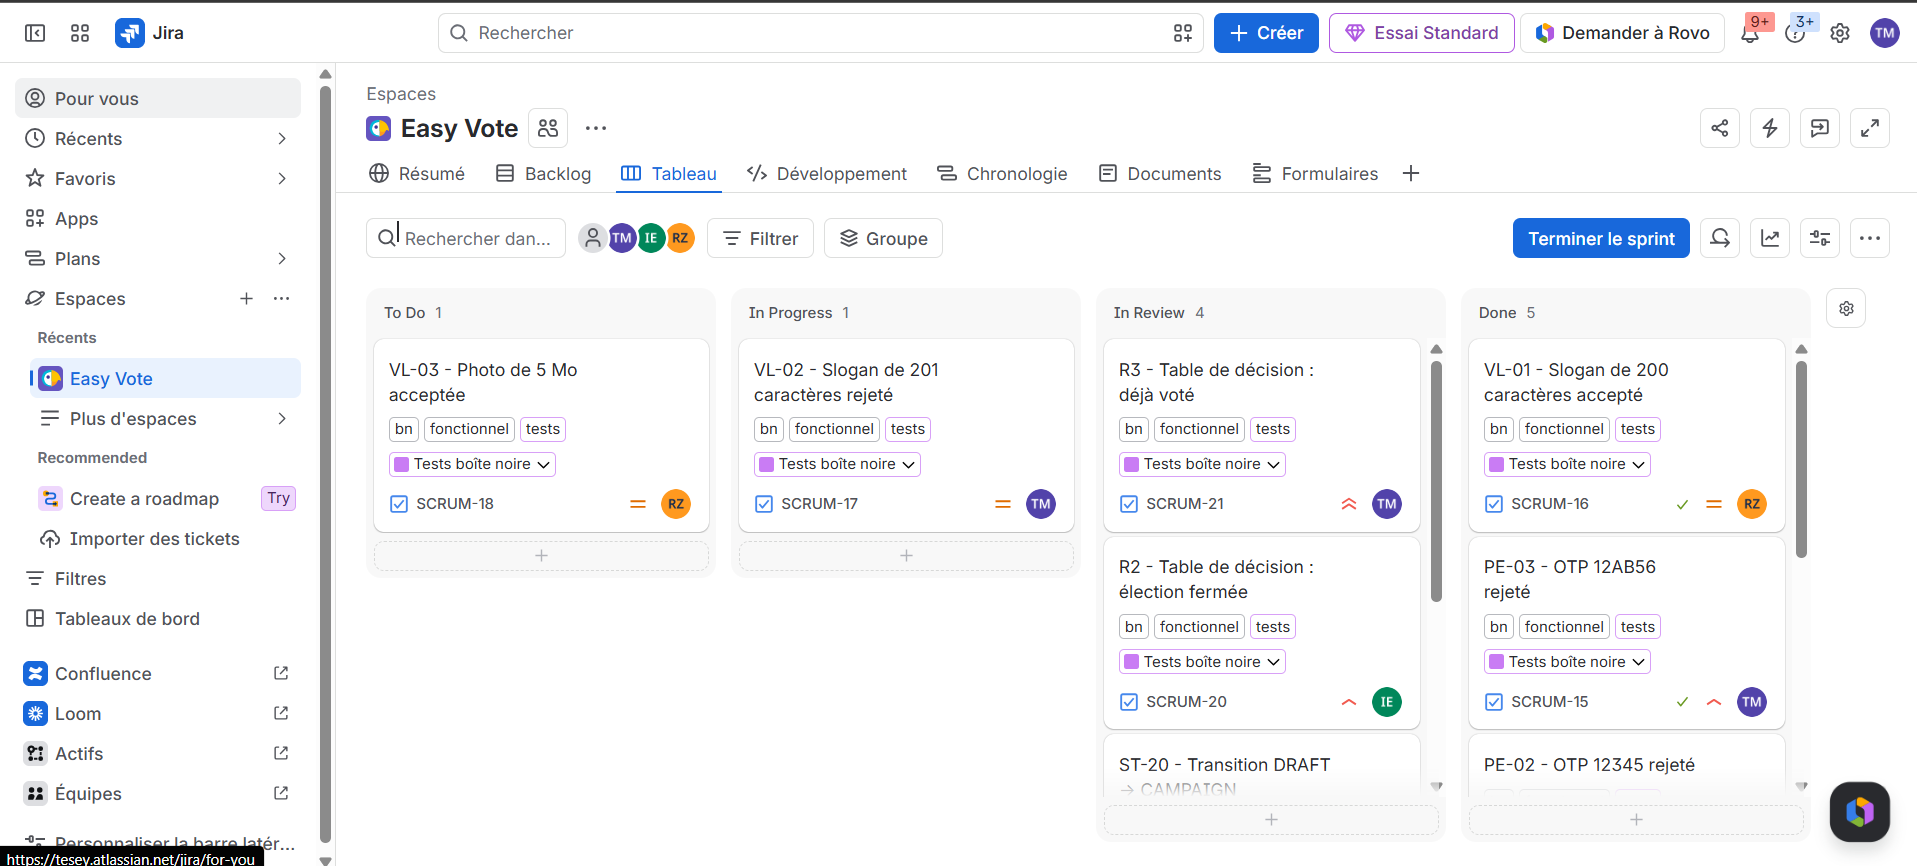
\includegraphics[width=\textwidth]{images/jira-tableau.png}
\caption{Jira --- tableau Scrum du sprint 1 : colonnes To Do, In Progress, In Review et Done}\label{fig:jira-tableau}
\end{figure}

\section{Rôle de chaque outil}
Les outils se complètent : Jira répond à la question « qui fait quoi, et où en est-on ? », Testiny à « quels cas de test, avec quel résultat ? ».

\begin{table}[H]
\centering
\caption{Répartition des rôles entre les outils de l'équipe}
\small
\begin{tabularx}{\textwidth}{@{}p{2.6cm}p{5cm}X@{}}
\toprule
\rowcolor{evlight}\textbf{Outil} & \textbf{Rôle} & \textbf{Contenu}\\
\midrule
Jira & Organisation du travail & Backlog, sprint, tableau d'avancement, bugs, responsables\\
Testiny & Gestion des tests & Cas de test, plans, exécutions, résultats, exigences (chapitre~\ref{ch:outil})\\
GitHub & Versionnement & Code source et tests automatisés\\
JUnit, scripts & Exécution des tests & Suite automatisée relançable en une commande\\
\bottomrule
\end{tabularx}
\end{table}

% ======================================================
\chapter{Besoins Fonctionnels et Non Fonctionnels}\label{ch:besoins}

\section{Besoins Fonctionnels}

\subsection{Étudiant}
\textbf{Compte et accès}
\begin{itemize}
  \item S'inscrire (nom, email, mot de passe) et activer son compte via un code OTP à 6 chiffres
  \item S'authentifier (JWT : access token 1\,h, refresh token 7 jours)
\end{itemize}
\textbf{Élections et candidatures}
\begin{itemize}
  \item Consulter les élections et la liste des candidats validés (slogan, programme)
  \item Postuler comme candidat lorsque l'élection est en statut \texttt{CAMPAIGN\_ACTIVE} (slogan $\leq$ 200 caractères, programme $\leq$ 5000 caractères, photo JPG/PNG $\leq$ 5\,Mo)
\end{itemize}
\textbf{Vote}
\begin{itemize}
  \item Voter une seule fois lorsque l'élection est en statut \texttt{VOTE\_ACTIVE}, avec étape de confirmation explicite
  \item Recevoir un code de confirmation à 10 caractères sans révéler son choix
  \item Consulter uniquement les statistiques de participation pendant le vote, puis les résultats détaillés après clôture
\end{itemize}
\textbf{Engagement et accompagnement}
\begin{itemize}
  \item Liker un candidat (toggle), commenter, poser des questions
  \item Dialoguer avec le chatbot EasyBot
  \item Consulter et marquer comme lues ses notifications
\end{itemize}

\subsection{Candidat}
\begin{itemize}
  \item Tous les droits de l'étudiant
  \item Modifier son programme et publier des annonces de campagne
  \item Répondre aux questions des étudiants
  \item Consulter ses statistiques d'engagement (tableau de bord « Ma campagne »)
\end{itemize}

\subsection{Administrateur}
\begin{itemize}
  \item Créer, modifier, supprimer des élections et gérer leur cycle de vie (\texttt{DRAFT} $\rightarrow$ \texttt{CAMPAIGN\_ACTIVE} $\rightarrow$ \texttt{VOTE\_ACTIVE} $\rightarrow$ \texttt{CLOSED})
  \item Valider ou rejeter les candidatures (avec note de rejet) ; le rôle passe alors de \texttt{STUDENT} à \texttt{CANDIDATE}
  \item Déclencher la génération (idempotente) des jetons de vote
  \item Consulter les statistiques détaillées temps réel (votes par heure, classement live)
  \item Générer et télécharger le rapport PDF officiel après clôture
  \item Gérer les utilisateurs
\end{itemize}

\section{Besoins Non Fonctionnels}

\paragraph{Performance.} Chargement initial $<$ 2\,s ; latence API en lecture $<$ 200\,ms ; chatbot (règles) $<$ 50\,ms et réponse IA $<$ 3\,s ; rafraîchissement des notifications toutes les 30\,s (paramétrable).

\paragraph{Sécurité.} Authentification JWT stateless ; mots de passe hachés (BCrypt, cost factor 10) ; endpoints protégés par \texttt{@PreAuthorize} (hiérarchie ADMIN $>$ CANDIDATE $>$ STUDENT) ; validation systématique des entrées (Bean Validation, react-hook-form) ; CORS strict ; mots de passe jamais retournés ni journalisés.

\paragraph{Anonymat et intégrité du vote.} Aucune référence à \texttt{user\_id} dans la table \texttt{votes} ; jeton haché en SHA-256, seul le hash étant stocké ; aucune requête SQL ne doit pouvoir relier un électeur à son vote ; un seul vote par électeur ; génération des jetons idempotente.

\paragraph{Maintenabilité.} Architecture en couches (Controller / Service / Repository) ; gestion centralisée des erreurs (\texttt{GlobalExceptionHandler}) ; conventions de nommage cohérentes.

\paragraph{Accessibilité et ergonomie.} Interface responsive mobile-first ; mode sombre/clair persistant ; composants shadcn/ui (Radix UI, ARIA) ; animations respectant \texttt{prefers-reduced-motion} ; français en V1.

\paragraph{Évolutivité.} Backend stateless scalable horizontalement ; ajout d'un fournisseur IA pour le chatbot par simple configuration.

\section{Exigences identifiées et traçabilité}
Pour permettre la gestion des exigences dans l'outil de test, les besoins ont été regroupés en 15 exigences identifiées (\texttt{EX-xx}). Chaque cas de test exécuté est rattaché à au moins une exigence.

{\small
\begin{longtable}{@{}p{1.1cm}p{6.2cm}p{2cm}p{4.2cm}p{1.4cm}@{}}
\caption{Matrice de traçabilité exigences $\rightarrow$ tests exécutés}\label{tab:trace}\\
\toprule
\rowcolor{evlight}\textbf{ID} & \textbf{Exigence} & \textbf{Source CDC} & \textbf{Tests exécutés} & \textbf{Verdict}\\
\midrule \endfirsthead
\toprule
\rowcolor{evlight}\textbf{ID} & \textbf{Exigence} & \textbf{Source CDC} & \textbf{Tests exécutés} & \textbf{Verdict}\\
\midrule \endhead
\bottomrule \endlastfoot
EX-01 & Inscription et activation par code OTP à 6 chiffres & §4.4.1, UC-01 & PE-01..03, IT-01 & \ok\\
EX-02 & Authentification JWT (access 1\,h, refresh 7\,j) & §4.4.1 & PM-01, PM-03, JWT-01 & \ko\\
EX-03 & Contrôle d'accès par rôle ; l'admin ne vote pas & §4.4.1, §6.1 & IT-09, PM-02, EX-3 & \ko\\
EX-04 & Cycle de vie d'une élection & §3.1.1 & ST-20, ST-21, ST-23, DC-01..03 & \ok\\
EX-05 & Candidature : statut, slogan $\leq$ 200, photo $\leq$ 5\,Mo & §3.1.2 & VL-01..03, EX-1 & \ko\\
EX-06 & Validation de candidature et passage au rôle CANDIDATE & §3.1.2 & ST-01, EX-2 & \ko\\
EX-07 & Génération idempotente des jetons (SHA-256) & §3.2.1 & UT-01a..c, B1..B3 & \ok\\
EX-08 & Un seul vote par électeur & §3.2.2 & R1..R3, ST-02 & \ok\\
EX-09 & Anonymat : aucun lien SQL électeur $\leftrightarrow$ vote & §3.2.2, §4.4.2 & IT-04, SQL-01, CC-3 & \ko\\
EX-10 & Code de confirmation à 10 caractères & §3.2.2 & R1, ST-01 & \ok\\
EX-11 & Transparence des résultats selon le statut & §3.2.3 & ST-03 & \ok\\
EX-12 & Export du rapport PDF officiel & §3.2.4 & ST-05 & \ok\\
EX-13 & Chatbot : réponses par règles en $<$ 50\,ms & §3.3.1, §5.1 & UT-01 (chatbot), UT-06, ex-UT-CB3 & \ko\\
EX-14 & Latence API en lecture $<$ 200\,ms & §5.1 & ST-NF, PM-02, ST-08 (JMeter) & \ko\\
EX-15 & Sauvegarde et restauration des données & §5.5 & MT-01, MT-02 & \ok\\
\end{longtable}
}

% ======================================================
\chapter{Outil de Gestion des Tests : Testiny}\label{ch:outil}

\section{Choix de l'outil}
Avant de retenir Testiny, l'équipe a évalué deux outils open source de gestion des tests, \textbf{TestLink} puis \textbf{Kiwi TCMS}, tous deux à installer sur un serveur local. Elle a finalement retenu \textbf{Testiny}, outil en ligne (SaaS), pour gérer à la fois les cas de test, les plans, les exécutions et leur rattachement aux exigences. Le tableau~\ref{tab:benchmark} résume la comparaison.

\begin{table}[H]
\centering
\caption{Comparaison des outils de gestion des tests évalués (appréciation qualitative de l'équipe, sans mesure de performance)}\label{tab:benchmark}
\small
\begin{tabularx}{\textwidth}{@{}>{\raggedright\arraybackslash}p{2.9cm}>{\raggedright\arraybackslash}X>{\raggedright\arraybackslash}X>{\raggedright\arraybackslash}X@{}}
\toprule
\rowcolor{evlight}\textbf{Critère} & \textbf{TestLink} & \textbf{Kiwi TCMS} & \textbf{Testiny}\\
\midrule
Licence / offre & Open source (GPL) & Open source (GPL) & SaaS ; offre gratuite pour une petite équipe\\
Déploiement & Serveur local : Apache, PHP, MySQL & Serveur local : Docker, MariaDB, HTTPS & Aucun : navigateur web\\
Mise en route & Longue (installation, configuration) & Moyenne (conteneurs, certificat) & Immédiate (compte en ligne)\\
Interface & Datée & Moderne mais dense & Moderne et épurée\\
Travail à trois & Comptes à créer sur notre serveur & Comptes à créer sur notre serveur & Invitation par email, accès simultané\\
Exigences & Module d'exigences intégré & Liens vers les anomalies, pas de module d'exigences dédié & Exigence notée dans chaque cas (EX-xx)\\
Intégration Jira & Oui (suivi d'anomalies) & Oui (suivi d'anomalies) & Oui\\
Résultats automatisés & API XML-RPC & API JSON-RPC et XML-RPC & Module \textit{Automation} (API)\\
Entretien de l'outil & À notre charge (mises à jour, sauvegardes) & À notre charge & Aucun\\
Coût pour le projet & Gratuit & Gratuit & Gratuit\\
\midrule
\textbf{Décision} & \textcolor{kored}{\textbf{Écarté}} & \textcolor{kored}{\textbf{Écarté}} & \textcolor{okgreen}{\textbf{Retenu}}\\
\bottomrule
\end{tabularx}
\end{table}

Les deux outils open source sont complets mais demandent d'installer et d'entretenir un serveur, ce qui n'apporte rien à un projet de trois personnes. Testiny offre le même cycle (cas, plans, exécutions, résultats) sans aucune installation.

\section{Justification du choix}
\begin{itemize}
  \item \textbf{Aucune installation} : application web accessible depuis un navigateur, contrairement à Kiwi TCMS qui nécessite Docker, une base MariaDB et un certificat local.
  \item \textbf{Travail collaboratif} : les trois membres travaillent en même temps sur le même projet, chacun avec son compte.
  \item \textbf{Organisation claire} : cas de test rangés en dossiers (un par niveau de test), avec identifiants automatiques (\texttt{TC-xx}, \texttt{TCF-x}).
  \item \textbf{Cycle complet} : cas de test $\rightarrow$ plans de test $\rightarrow$ exécutions (\textit{test runs}) $\rightarrow$ résultats (Passed, Failed, Blocked, Skipped, Not Run).
  \item \textbf{Suivi} : tableau de bord, jalons (\textit{milestones}) et module \textit{Automation} pour rattacher des résultats de tests automatisés.
  \item \textbf{Traçabilité} : chaque cas de test contient l'identifiant de l'exigence couverte (\texttt{EX-xx}) et les défauts sont liés aux exécutions en échec.
\end{itemize}

\section{Configuration du projet EasyVote dans Testiny}
\begin{enumerate}
  \item Création de l'organisation et du projet \textbf{easyvote}, et invitation des trois membres de l'équipe.
  \item Création d'un dossier par niveau de test, reprenant le plan du chapitre~\ref{ch:plan} : \textbf{Unitaire} (12 cas), \textbf{Intégration} (24 cas), \textbf{Système (E2E)} (22 cas), \textbf{Acceptation (UAT)} (10 cas), soit \textbf{68 cas de test}.
  \item Saisie de chaque cas : titre préfixé par sa référence (UT-01, IT-04, ST-01\ldots), préconditions, étapes, résultat attendu, priorité et exigence couverte.
  \item Création des \textbf{test runs} (un par niveau) pour l'exécution, puis saisie du résultat de chaque cas et du défaut associé en cas d'échec.
\end{enumerate}

\begin{figure}[H]
\centering
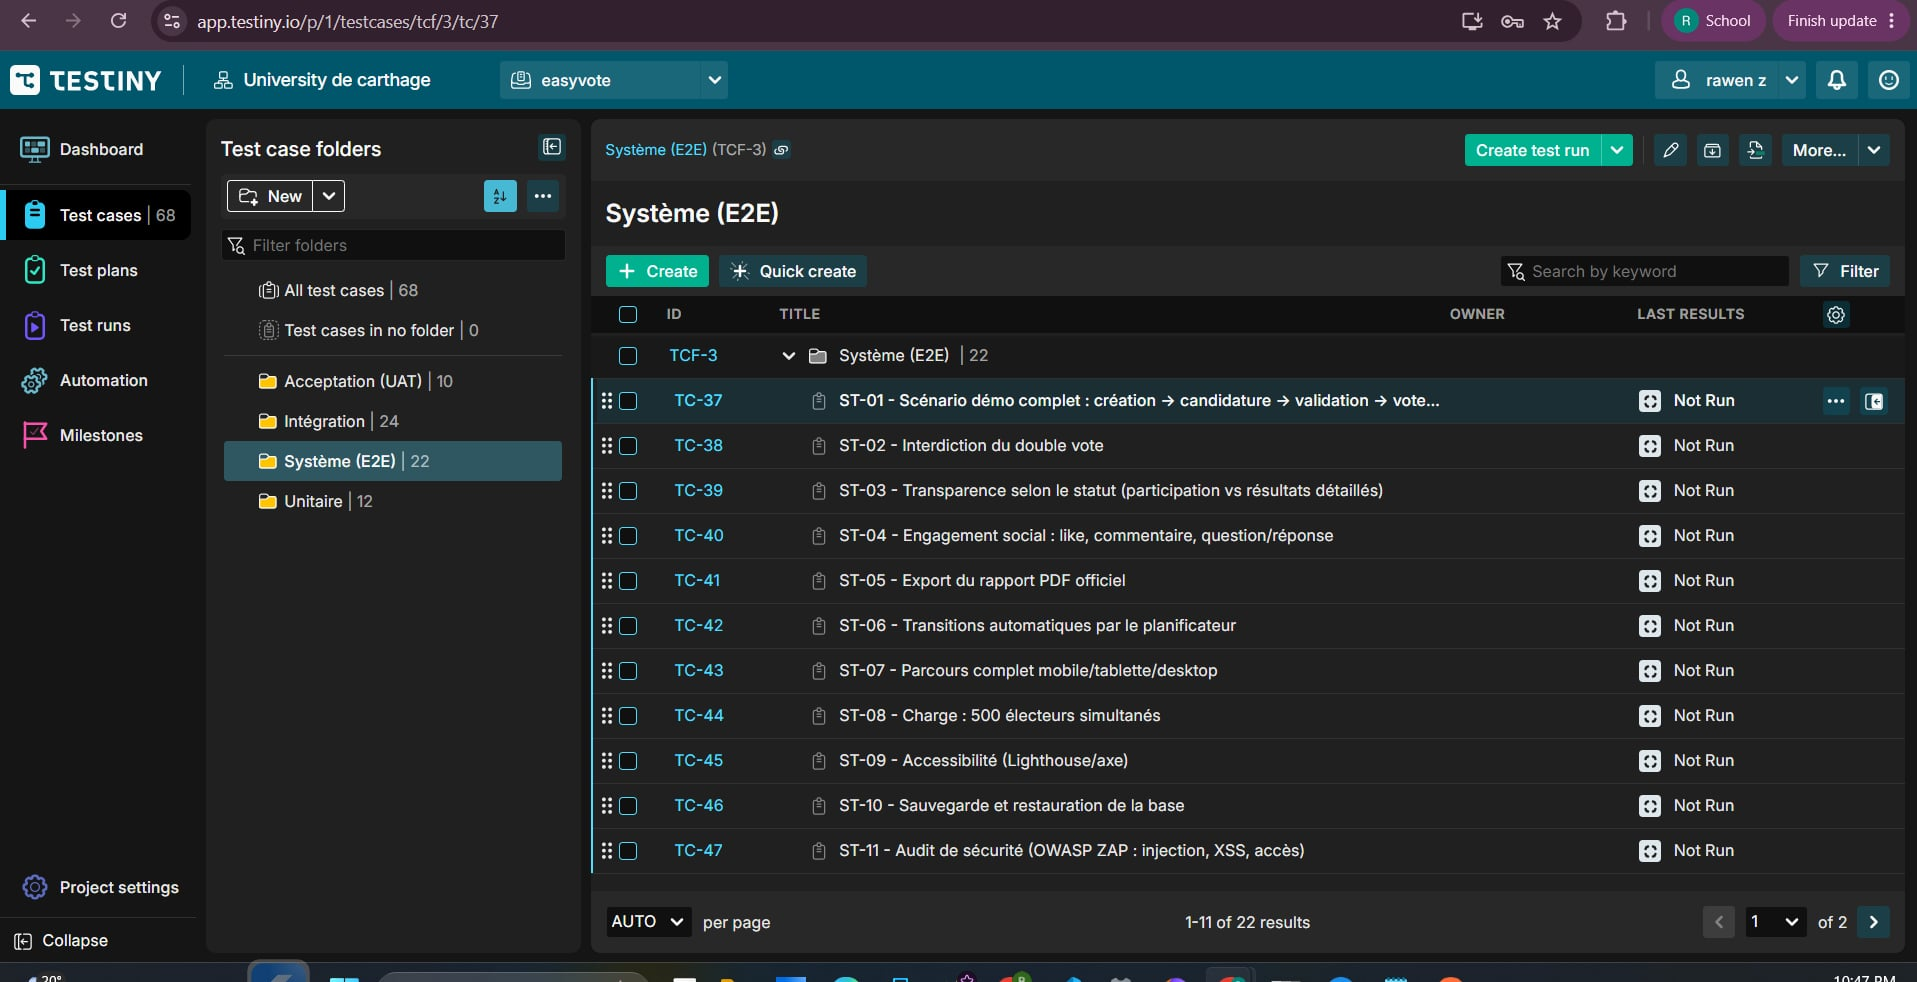
\includegraphics[width=\textwidth]{images/testiny-cas-de-test.jpg}
\caption{Testiny --- projet easyvote : 68 cas de test répartis en 4 dossiers (niveaux), dossier Système (E2E) ouvert}
\end{figure}


% ======================================================
\chapter{Plan de Test}\label{ch:plan}

\section{Stratégie de test}
La stratégie est \textbf{basée sur les risques} : les fonctions dont l'échec aurait l'impact le plus fort (anonymat, vote unique, contrôle d'accès) reçoivent la priorité \textit{Critique} et sont testées en premier, à plusieurs niveaux et avec plusieurs techniques.

\begin{table}[H]
\centering
\caption{Risques métier principaux et réponse de test}
\small
\begin{tabularx}{\textwidth}{@{}Xp{1.8cm}X@{}}
\toprule
\rowcolor{evlight}\textbf{Risque} & \textbf{Niveau} & \textbf{Réponse de test}\\
\midrule
Un électeur peut être relié à son vote & Critique & IT-04, SQL-01, revue du modèle de données\\
Un étudiant vote deux fois & Critique & Table de décision R1..R3, ST-02\\
Un utilisateur accède à une fonction d'un autre rôle & Critique & IT-09, PM-02, test exploratoire EX-3\\
Résultats divulgués pendant le vote & Haute & ST-03\\
Saisies invalides acceptées (OTP, slogan, photo) & Haute & Partitions d'équivalence, valeurs limites\\
Lenteur de l'API ou du chatbot & Moyenne & UT-06, ST-NF, PM-02\\
\bottomrule
\end{tabularx}
\end{table}

\section{Niveaux et types de tests}
Le plan couvre les \textbf{quatre niveaux} (unitaire, intégration, système, acceptation) et les \textbf{types} suivants : \textbf{fonctionnels} (le système fait-il ce qui est attendu ?), \textbf{non fonctionnels} (performance, sécurité, utilisabilité), \textbf{structurels} (couverture du code), \textbf{liés aux changements} (tests de confirmation et de régression) et de \textbf{maintenance} (sauvegarde, migration, mise à jour).

\begin{table}[H]
\centering
\caption{Répartition des 68 cas du plan par niveau et par type}
\small
\begin{tabular}{@{}lccccc@{}}
\toprule
\rowcolor{evlight}\textbf{Niveau} & \textbf{Fonct.} & \textbf{Non-fonct.} & \textbf{Struct.} & \textbf{Régr. / Maint.} & \textbf{Total}\\
\midrule
Unitaire & 5 & 2 & 2 & 3 & 12\\
Intégration & 11 & 3 & 4 & 6 & 24\\
Système (E2E) & 7 & 4 & 1 & 10 & 22\\
Acceptation (UAT) & 4 & 2 & 1 & 3 & 10\\
\midrule
\textbf{Total} & 27 & 11 & 8 & 22 & \textbf{68}\\
\bottomrule
\end{tabular}
\end{table}

\section{Outils de test retenus}
Quatre outils principaux couvrent les niveaux et les types du plan. Ils sont complétés par des outils légers pour les vérifications ponctuelles.

\begin{table}[H]
\centering
\caption{Outils de test par niveau, type et technique}
\small
\begin{tabularx}{\textwidth}{@{}p{2.2cm}p{3cm}p{3.4cm}X@{}}
\toprule
\rowcolor{evlight}\textbf{Outil} & \textbf{Niveaux} & \textbf{Types} & \textbf{Technique et utilisation}\\
\midrule
\textbf{JUnit 5} (+ Mockito, JaCoCo) & Unitaire, intégration & Fonctionnel, structurel, régression & Dynamique, boîte noire et boîte blanche ; couverture mesurée par JaCoCo ; automatisé\\
\textbf{Postman} (+ Newman) & Intégration, système & Fonctionnel, non fonctionnel (sécurité) & Dynamique, boîte noire sur l'API REST ; collection rejouable ; automatisé\\
\textbf{SonarQube} & Code (tous niveaux) & Structurel, maintenabilité, sécurité & Statique : bugs, vulnérabilités, \textit{code smells}, complexité, duplication ; automatisé\\
\textbf{JMeter} & Système & Non fonctionnel (performance, charge) & Dynamique : utilisateurs simultanés, assertions de temps de réponse ; automatisé\\
\midrule
jwt.io, SQL, navigateur & Intégration, système, acceptation & Fonctionnel, sécurité, utilisabilité & Vérifications manuelles (jeton, anonymat, exploratoire, UAT)\\
ESLint, tsc, npm audit & Code frontend & Structurel, sécurité & Statique outillée\\
Testiny & Tous & Tous & Gestion des cas, exécutions, résultats et défauts\\
Jira & Tous & --- & Organisation du travail : backlog, sprint, tableau, bugs (chapitre~\ref{ch:jira})\\
\bottomrule
\end{tabularx}
\end{table}

\paragraph{Critères d'entrée de l'exécution.} Application compilée et démarrée (backend, base MariaDB, frontend), jeu de données de test chargé (\texttt{tests/seed-demo.sql}), cas de test saisis dans Testiny.

\paragraph{Critères de sortie.} Tous les cas \textit{Critique} exécutés ; chaque échec enregistré comme défaut et rattaché à son cas de test ; aucune régression sur les tests déjà réussis.

\section{Cas de test par niveau}
Chaque niveau est détaillé selon les colonnes : Référence, Type (Fonct. = Fonctionnel, Non-fonct. = Non-fonctionnel, Struct. = Structurel, Régr. = Régression / maintenance), Scénario, Priorité, Données de test, Résultat attendu et \textbf{Résultat} de l'exécution (chapitre~\ref{ch:execution}) : \ok, \ko, \pa\ (exécuté en partie) ou \nex.

{\footnotesize
\setlength{\tabcolsep}{4pt}
% ---------------------------------------------------------------------
\subsection{Niveau Unitaire}

\begin{longtable}{@{}p{1.45cm}p{1.25cm}p{2.9cm}p{1.15cm}p{2.3cm}p{3.4cm}p{1.6cm}@{}}
\caption{Plan de test --- Niveau Unitaire}\\
\toprule \planHead \\ \midrule \endfirsthead
\toprule \planHead \\ \midrule \endhead
\bottomrule \endlastfoot
UT-01 & Fonct. & \texttt{hashToken()} : SHA-256 d'un jeton & Critique & jeton fixe, vecteur NIST & Hash de 64 caractères hexadécimaux, déterministe, différent du jeton & \ok\\
UT-02 & Fonct. & Génération du code de confirmation & Haute & vote valide & Code de 10 caractères, sans doublon & \pa\\
UT-03 & Fonct. & Hachage du mot de passe (BCrypt) & Moyenne & mdp = \texttt{Test@1234} & Hash $\neq$ clair, préfixe \texttt{\$2a\$} & \ok\\
UT-04 & Fonct. & Génération et expiration du code OTP & Haute & code généré à $t$, test à $t$+9 et $t$+11 min & 6 chiffres ; valide à 9 min, expiré à 11 min & \nex\\
UT-05 & Fonct. & Décodage d'un token JWT valide & Critique & token réel décodé (jwt.io) & Rôle et expiration conformes (access 1\,h / refresh 7 j) & \ko\\
UT-06 & Non-fonct. & Temps de réponse du chatbot (couche règles) & Moyenne & question « Comment voter ? » & $<$ 50 ms & \ok\\
UT-07 & Non-fonct. & Complexité cyclomatique de \texttt{castVote()} & Basse & SonarQube + calcul de V(G) & $\leq$ seuil défini (10) & \ko\\
UT-08 & Struct. & Couverture des branches des transitions d'état & Haute & 2 transitions valides + 1 illégale & 100\,\% des branches couvertes & \pa\\
UT-09 & Struct. & Exceptions métier du vote & Haute & déjà voté, élection non active & Exceptions métier levées, aucun vote enregistré & \ok\\
UT-M01 & Régr. & Non-régression du calcul des résultats après refactoring & Haute & jeu de votes de référence & Résultat identique avant/après & \ok\\
UT-M02 & Régr. & Compatibilité ascendante des DTO & Moyenne & ancien payload JSON & Désérialisation OK, valeur par défaut & \nex\\
UT-M03 & Régr. & Couverture de tests après modification d'un service & Haute & rapport JaCoCo avant/après & Couverture maintenue $\geq$ 70\,\% & \nex\\
\end{longtable}

\textit{Remarques.} UT-02 : le format (10 caractères \texttt{[A-Z0-9]}) est vérifié par R1, pas l'absence de doublon. UT-05 : le jeton dure 24\,h (DEF-06). UT-07 : V(G) = 12 $>$ 10. UT-08 : la transition VOTE\_ACTIVE $\rightarrow$ CLOSED n'a pas été testée. UT-M01 : exécuté en JUnit (\texttt{RegressionResultatsTest}) sur un jeu de 10 votes de référence ; il sert de filet de sécurité lors d'un refactoring.

% ---------------------------------------------------------------------
\subsection{Niveau Intégration}

\begin{longtable}{@{}p{1.45cm}p{1.25cm}p{2.9cm}p{1.15cm}p{2.3cm}p{3.4cm}p{1.6cm}@{}}
\caption{Plan de test --- Niveau Intégration}\\
\toprule \planHead \\ \midrule \endfirsthead
\toprule \planHead \\ \midrule \endhead
\bottomrule \endlastfoot
IT-01 & Fonct. & \texttt{POST /auth/register} $\leftrightarrow$ email OTP $\leftrightarrow$ BDD & Haute & nom, email, mdp valides & Compte \texttt{STUDENT} non vérifié créé, email OTP envoyé & \ok\\
IT-02 & Fonct. & \texttt{POST /auth/login} $\leftrightarrow$ MariaDB & Haute & utilisateur vérifié + bon mdp & HTTP 200 + JWT (access + refresh) & \ok\\
IT-03 & Fonct. & Génération des jetons $\leftrightarrow$ \texttt{vote\_tokens} (idempotence) & Critique & élection + étudiants, 2 lancements & 1 hash par électeur, 2\textsuperscript{e} lancement sans effet & \ok\\
IT-04 & Fonct. & POST \nolinkurl{/elections/{id}/vote} $\leftrightarrow$ table \texttt{votes} (anonymat) & Critique & jeton valide, candidat validé & Pas de \texttt{user\_id}, aucune jointure possible ; code retourné & \ko\\
IT-05 & Fonct. & Chatbot $\leftrightarrow$ API IA externe (fallback) & Moyenne & question hors FAQ & Réponse IA reçue et affichée & \nex\\
IT-06 & Fonct. & Validation d'une candidature $\leftrightarrow$ rôle $\leftrightarrow$ notification & Haute & candidature \texttt{PENDING} & Statut \texttt{VALIDATED}, rôle \texttt{CANDIDATE}, notification & \ok\\
IT-07 & Non-fonct. & Temps de réponse \texttt{GET /elections} & Moyenne & 20 appels successifs & $\leq$ 200 ms & \ok\\
IT-08 & Non-fonct. & Résilience si l'API IA est indisponible & Critique & timeout simulé & Repli sur les règles, aucune erreur 500 & \nex\\
IT-09 & Struct. & Filtre JWT et \texttt{@PreAuthorize} & Critique & sans token ; \texttt{STUDENT} sur endpoint \texttt{ADMIN} & 401 puis 403 & \ok\\
IT-10 & Struct. & Contraintes d'unicité en base & Haute & 2\textsuperscript{e} like ; \texttt{token\_hash} dupliqué & Insertions rejetées, erreur gérée & \nex\\
IT-11 & Fonct. & \texttt{POST /auth/refresh} & Haute & refresh token valide & Nouvel access token émis & \nex\\
IT-12 & Fonct. & \texttt{GET /elections} $\leftrightarrow$ JPA $\leftrightarrow$ MariaDB & Haute & élections en base & Liste paginée, tri par date & \pa\\
IT-13 & Fonct. & Upload photo de candidature $\leftrightarrow$ stockage & Haute & photo JPG $\leq$ 5 Mo & Fichier stocké, URL retournée & \nex\\
IT-14 & Fonct. & \texttt{GET /results} $\leftrightarrow$ agrégation SQL & Critique & votes en base & Totaux et pourcentages exacts & \ok\\
IT-15 & Fonct. & Marquer une notification comme lue & Moyenne & notification existante & Statut \texttt{read}, badge décrémenté & \nex\\
IT-16 & Non-fonct. & Rollback sur vote échoué & Critique & erreur simulée après insert & Aucune ligne partielle, jetons intacts & \nex\\
IT-17 & Struct. & Contrainte FK candidat $\rightarrow$ élection & Moyenne & suppression élection avec candidats & Cascade ou rejet selon règle & \nex\\
IT-18 & Struct. & Index sur \texttt{votes} & Moyenne & EXPLAIN sur requête & Index utilisés & \nex\\
IT-M01 & Régr. & Migration de schéma (ajout de colonne) & Haute & script + base peuplée & Pas de perte de données & \nex\\
IT-M02 & Régr. & Rollback de migration & Critique & échec simulé & Retour à l'état antérieur & \nex\\
IT-M03 & Régr. & Nouveau format de réponse de l'API IA & Haute & mock nouvelle réponse & Parsing adapté & \nex\\
IT-M04 & Régr. & Montée de version Spring Boot & Moyenne & benchmark avant/après & Aucune dégradation & \nex\\
IT-M05 & Régr. & Compatibilité des endpoints après ajout & Haute & collection Postman rejouée & Aucun breaking change & \nex\\
IT-M06 & Régr. & Non-régression de l'anonymat & Critique & schéma + données après vote & Aucune colonne ni jointure vers \texttt{user\_id} & \ko\\
\end{longtable}

\textit{Remarques.} IT-02 et IT-07 ont été exécutés via Postman et le script système. IT-06 : l'état final est correct mais le rôle change trop tôt (DEF-02, test exploratoire EX-2). IT-12 : la liste est triée mais non paginée. IT-05 et IT-08 : fournisseur IA désactivé dans la configuration.

% ---------------------------------------------------------------------
\subsection{Niveau Système (E2E)}

\begin{longtable}{@{}p{1.45cm}p{1.25cm}p{2.9cm}p{1.15cm}p{2.3cm}p{3.4cm}p{1.6cm}@{}}
\caption{Plan de test --- Niveau Système}\\
\toprule \planHead \\ \midrule \endfirsthead
\toprule \planHead \\ \midrule \endhead
\bottomrule \endlastfoot
ST-01 & Fonct. & Scénario démo : création $\rightarrow$ candidature $\rightarrow$ validation $\rightarrow$ vote $\rightarrow$ résultats & Critique & admin, 2 étudiants, 1 élection & Parcours sans erreur, résultats corrects & \ok\\
ST-02 & Fonct. & Interdiction du double vote & Critique & étudiant ayant déjà voté & 2\textsuperscript{e} vote refusé, message clair & \ok\\
ST-03 & Fonct. & Transparence selon le statut & Critique & élection \texttt{VOTE\_ACTIVE} puis \texttt{CLOSED} & Participation seule pendant le vote ; détails après & \ok\\
ST-04 & Fonct. & Engagement social : like, commentaire, Q/R & Moyenne & étudiant + candidat & Actions visibles, notifications & \nex\\
ST-05 & Fonct. & Export du rapport PDF officiel & Haute & élection \texttt{CLOSED} & PDF valide et complet & \ok\\
ST-06 & Fonct. & Transitions automatiques (planificateur) & Haute & dates proches & Statuts mis à jour & \nex\\
ST-07 & Fonct. & Parcours mobile / tablette / desktop & Moyenne & 3 résolutions & Affichage cohérent & \nex\\
ST-08 & Non-fonct. & Charge : 500 électeurs simultanés & Haute & scénario JMeter & $\leq$ 200 ms, aucune erreur & \ko\\
ST-09 & Non-fonct. & Accessibilité (Lighthouse/axe) & Moyenne & pages clés & Aucune erreur bloquante & \nex\\
ST-10 & Non-fonct. & Sauvegarde et restauration de la base & Haute & sauvegarde + restauration & Données restaurées à l'identique & \ok\\
ST-11 & Non-fonct. & Audit de sécurité & Haute & SonarQube (code) ; OWASP ZAP (API) & Aucune vulnérabilité critique & \pa\\
ST-12 & Struct. & Cohérence rôles/menus par profil & Haute & 3 connexions & Interface conforme au rôle & \nex\\
REG-00-1 & Régr. & Connexion des 3 rôles (socle) & Critique & 3 comptes de test & JWT et rôle corrects & \ok\\
REG-00-2 & Régr. & Workflow de vote (socle) & Critique & élection \texttt{VOTE\_ACTIVE} & Vote enregistré, code & \ok\\
REG-00-3 & Régr. & Accès RBAC croisé (socle) & Critique & 3 rôles $\times$ endpoints & 403 si non autorisé & \pa\\
REG-00-4 & Régr. & Anonymat de la table \texttt{votes} (socle) & Critique & schéma + données & Aucune colonne ni jointure vers \texttt{user\_id} & \ko\\
REG-00-5 & Régr. & Temps de réponse des endpoints critiques & Haute & 20 appels & $\leq$ 200 ms & \ok\\
ST-M01 & Régr. & Non-régression du module Vote après correctif & Critique & suite ST-01 à ST-03 & Tous les scénarios passent & \nex\\
ST-M02 & Régr. & Déploiement sans interruption & Haute & rolling/blue-green & Disponibilité maintenue & \nex\\
ST-M03 & Régr. & Restauration après incident & Critique & sauvegarde + incident & Plateforme cohérente & \nex\\
ST-M04 & Régr. & Ajout d'un fournisseur IA & Moyenne & nouveau provider & Chatbot intact & \nex\\
ST-M05 & Régr. & Compatibilité multi-navigateurs & Moyenne & Chrome, Firefox, Safari & Rendu identique & \nex\\
\end{longtable}

\textit{Remarques.} ST-08 : à 500 utilisateurs, toutes les réponses sont correctes (HTTP 200) mais plus de la moitié dépassent 200\,ms (DEF-08) ; à 200 utilisateurs l'exigence est respectée. ST-11 : le code a été audité par SonarQube (0 vulnérabilité) ; le scan dynamique OWASP ZAP n'a pas été réalisé. REG-00-3 : seul l'endpoint \texttt{/api/admin/users} a été testé, et l'admin peut voter (DEF-05). ST-M01 sera exécuté après correction des défauts.

% ---------------------------------------------------------------------
\subsection{Niveau Acceptation (UAT)}

\begin{longtable}{@{}p{1.45cm}p{1.25cm}p{2.9cm}p{1.15cm}p{2.3cm}p{3.4cm}p{1.6cm}@{}}
\caption{Plan de test --- Niveau Acceptation}\\
\toprule \planHead \\ \midrule \endfirsthead
\toprule \planHead \\ \midrule \endhead
\bottomrule \endlastfoot
UAT-01 & Fonct. & Étudiant : connexion $\rightarrow$ consultation $\rightarrow$ vote & Critique & compte \texttt{talel@test.com} & Parcours compris, code reçu & \ok\\
UAT-02 & Fonct. & Candidat gère sa campagne (programme, annonces, réponses) & Haute & compte \texttt{achref@test.com} & Ergonomie validée & \aex\\
UAT-03 & Fonct. & Administrateur crée une élection et traite les candidatures & Haute & compte \texttt{ahmed@test.com} & Processus clair, PDF obtenu & \aex\\
UAT-04 & Fonct. & Pertinence des réponses du chatbot & Moyenne & 10 questions d'étudiants & Réponses utiles et correctes & \aex\\
UAT-05 & Non-fonct. & Perception de la rapidité & Moyenne & questionnaire post-usage & Note moyenne $\geq$ 4/5 & \aex\\
UAT-06 & Non-fonct. & Clarté du PDF officiel & Moyenne & PDF réel & Validé comme exploitable & \ok\\
UAT-07 & Struct. & Rôles et droits conformes au besoin métier & Haute & test croisé des 3 rôles & Aucun accès incohérent & \ok\\
UAT-M01 & Régr. & Évolution demandée conforme au besoin & Haute & environnement de recette & Fonctionnalité conforme & \aex\\
UAT-M02 & Régr. & Procédure de maintenance planifiée & Moyenne & fenêtre simulée & Utilisateurs informés & \aex\\
UAT-M03 & Régr. & Rôles/droits inchangés après mise à jour & Haute & test croisé & Aucun changement non souhaité & \ok\\
\end{longtable}

\textit{Remarques.} UAT-01, UAT-06, UAT-07 et UAT-M03 ont été exécutés dans leur \textbf{version automatisée} (section~\ref{sec:uat-auto}). Les critères qui demandent un jugement humain (questionnaire, ergonomie, clarté du PDF) restent à valider manuellement, comme les autres cas d'acceptation.
}% fin footnotesize

% ======================================================
\chapter{Exécution du Plan de Test}\label{ch:execution}

\section{Organisation de l'exécution}
L'exécution combine des \textbf{techniques statiques} (revue, analyse outillée) et \textbf{dynamiques} (boîte noire, boîte blanche, exploratoire), des tests \textbf{automatisés} (rejouables en une commande) et \textbf{manuels}. Les résultats sont reportés dans les \textit{test runs} de Testiny.

\begin{table}[H]
\centering
\caption{Outils utilisés pendant l'exécution}
\small
\begin{tabularx}{\textwidth}{@{}p{4.2cm}X@{}}
\toprule
\rowcolor{evlight}\textbf{Outil} & \textbf{Usage}\\
\midrule
JUnit 5, AssertJ, Mockito & Tests unitaires boîte noire et boîte blanche (services isolés de la base)\\
Spring Boot Test, MockMvc, H2 & Tests d'intégration : application démarrée, sécurité JWT, base en mémoire\\
JaCoCo & Mesure de la couverture du code (preuve des techniques boîte blanche)\\
Postman / Newman & Tests d'API (connexion, profil \texttt{/auth/me}, sécurité)\\
jwt.io & Décodage manuel du contenu des jetons JWT\\
Script Node.js & Tests système de bout en bout sur l'API réelle\\
Apache JMeter 5.6.3 & Tests de charge et de performance (jusqu'à 500 utilisateurs simultanés)\\
SonarQube 10.6 (Docker) & Analyse statique de la qualité du code backend : bugs, vulnérabilités, \textit{code smells}, complexité, duplication, couverture\\
ESLint, tsc, npm audit & Analyse statique du frontend\\
MariaDB (XAMPP) & Base réelle pour les tests système, SQL et maintenance\\
Testiny & Gestion des cas, des exécutions et des résultats\\
Jira & Organisation du travail de l'équipe : backlog, sprint, tableau, bugs\\
\bottomrule
\end{tabularx}
\end{table}

Tous les tests automatisés se relancent depuis la racine du projet :
\begin{lstlisting}
.\tests\lancer-tests.ps1              # 38 tests JUnit (ou : boitenoire, boiteblanche, unitaire, integration, acceptation)
.\tests\lancer-tests.ps1 PE-01        # un seul test, par son identifiant
node tests/system-tests.mjs           # tests systeme de bout en bout
node tests/exploratoire.mjs           # tests exploratoires
.\tests\maintenance-sauvegarde.ps1    # test de maintenance
npx newman run tests/postman/EasyVote.postman_collection.json
\end{lstlisting}

% ------------------------------------------------------
\section{Techniques statiques}

Les techniques statiques n'exigent pas l'exécution du logiciel : elles trouvent les \textbf{causes} des défauts plutôt que les défaillances, et plus tôt, donc à moindre coût.

\subsection{Place des techniques statiques dans le projet}\label{sec:statique-cours}
Le tableau ci-dessous rapproche les techniques statiques du cours de leur usage dans EasyVote. Elles complètent les tests dynamiques : aucune des deux familles ne remplace l'autre.
\begin{table}[H]
\centering
\caption{Techniques statiques du cours et application dans EasyVote}
\small
\begin{tabularx}{\textwidth}{@{}p{3.6cm}X@{}}
\toprule
\rowcolor{evlight}\textbf{Technique (cours)} & \textbf{Application dans EasyVote}\\
\midrule
Revue informelle (entre pairs) & Relecture par un second membre avant le passage d'un ticket Jira de \textit{In Review} à \textit{Done}\\
Revue technique (formelle) & Revue du code contre le cahier des charges, avec checklist et constats numérotés RV-01 à RV-06 (ci-dessous)\\
Inspection & Non pratiquée : elle exige un modérateur formé et des critères d'entrée et de sortie formels, hors du périmètre de ce projet\\
Analyse statique outillée & SonarQube (backend) ; ESLint, tsc et npm audit (frontend)\\
\bottomrule
\end{tabularx}
\end{table}
Critère de sortie de la revue : chaque constat est consigné (RV-xx) et rattaché à un défaut DEF-xx ou à une observation.

\subsection{Revue technique}
La revue technique (formelle) a été menée selon le processus : planification, lancement, préparation individuelle, réunion de revue, re-travail et suivi. Les rôles (modérateur, auteur, réviseur, scribe) tournent entre les trois membres. La checklist a été dérivée du cahier des charges.

\begin{table}[H]
\centering
\caption{Résultats de la revue technique du code}
\small
\begin{tabularx}{\textwidth}{@{}p{1.1cm}p{4.3cm}Xp{1.8cm}@{}}
\toprule
\rowcolor{evlight}\textbf{Réf.} & \textbf{Point de contrôle (CDC)} & \textbf{Constat dans le code} & \textbf{Défaut}\\
\midrule
RV-01 & Access token valide 1\,h (§4.4.1) & \texttt{application.properties}, ligne 23 :\newline \texttt{easyvote.jwt.expiration=86400000} (24\,h) & DEF-06\\
RV-02 & Rôle CANDIDATE après validation (§3.1.2) & \texttt{CandidateService}, ligne 71 : rôle modifié dès le dépôt & DEF-02\\
RV-03 & Photo $\leq$ 5\,Mo (§3.1.2) & \texttt{PhotoUploadService}, ligne 34 : limite \texttt{5\_000\_000} octets ($\neq$ 5\,242\,880) & DEF-01\\
RV-04 & L'admin ne vote pas (§6.1) & \texttt{VoteService.castVote()} : aucun contrôle de rôle & DEF-05\\
RV-05 & Aucun lien SQL électeur $\leftrightarrow$ vote (§4.4.2) & même \texttt{token\_hash} dans \texttt{votes} et \texttt{vote\_tokens} & DEF-00\\
RV-06 & Aucun secret dans le dépôt & \texttt{application.properties} : identifiants SMTP en clair & Observation\\
\bottomrule
\end{tabularx}
\end{table}

Les constats RV-02, RV-04 et RV-05 ont ensuite été \textbf{confirmés dynamiquement} (sections~\ref{sec:anonymat} et~\ref{sec:explo}) : la revue a orienté les tests dynamiques.

\subsection{Analyse statique avec SonarQube (backend)}
SonarQube 10.6 (édition Community, lancé dans Docker) a analysé les 4\,875 lignes de code Java du backend, en important la couverture JaCoCo des tests JUnit. L'analyse se relance avec \texttt{tests/sonar-analyse.ps1}.

\begin{table}[H]
\centering
\caption{Résultats de l'analyse SonarQube}
\small
\begin{tabularx}{\textwidth}{@{}p{4.4cm}p{2.6cm}X@{}}
\toprule
\rowcolor{evlight}\textbf{Mesure} & \textbf{Valeur} & \textbf{Interprétation}\\
\midrule
Quality Gate (Sonar way) & Passed & première analyse : la règle porte sur le « nouveau code »\\
Vulnérabilités & 0 & note de sécurité A\\
Bugs & 3 & tous des \textbf{faux positifs} (voir ci-dessous)\\
Security hotspots & 2 & analysés et justifiés ci-dessous ; statut « Reviewed » non renseigné dans l'outil (0\,\%)\\
Code smells & 45 & note de maintenabilité A\\
Couverture & 35,3\,\% & lignes 38,0\,\% et branches 25,3\,\% (JaCoCo, 38 tests JUnit)\\
Duplication & 2,7\,\% & faible\\
Complexité cyclomatique & 460 & \texttt{ElectionService} 56, \texttt{ChatbotRulesService} 39, \texttt{VoteService} 22\\
\bottomrule
\end{tabularx}
\end{table}

\textbf{Tri des résultats} (étape indispensable d'une analyse statique) :
\begin{itemize}
  \item \textbf{3 bugs (règle S6857, « placeholder mal formé ») = faux positifs.} Les annotations visées, par exemple \texttt{@Value("\$\{easyvote.app.url:http://localhost:5173\}")}, ont une valeur par défaut contenant une URL avec \og : \fg. Spring utilise le premier \og : \fg\ comme séparateur : le code fonctionne.
  \item \textbf{Hotspot \og CSRF désactivé \fg} (\texttt{SecurityConfig}) : justifié, car l'API est stateless et authentifiée par JWT, ce que prévoit le cahier des charges (§5.2).
  \item \textbf{Hotspot \og expression régulière \fg} (\texttt{CorsConfig}) : sans risque, l'expression ne s'applique qu'à une valeur de configuration et jamais à une saisie utilisateur.
  \item \textbf{Complexité cognitive} : \texttt{ChatbotRulesService.tryMatchRule()} atteint 37 pour un maximum recommandé de 15. Cette méthode, une longue suite de règles évaluées dans l'ordre, est justement celle où l'ancien test UT-CB3 a trouvé DEF-04 : la complexité signalée par l'outil et le défaut trouvé par le test dynamique se confirment mutuellement.
\end{itemize}

\begin{figure}[H]
\centering
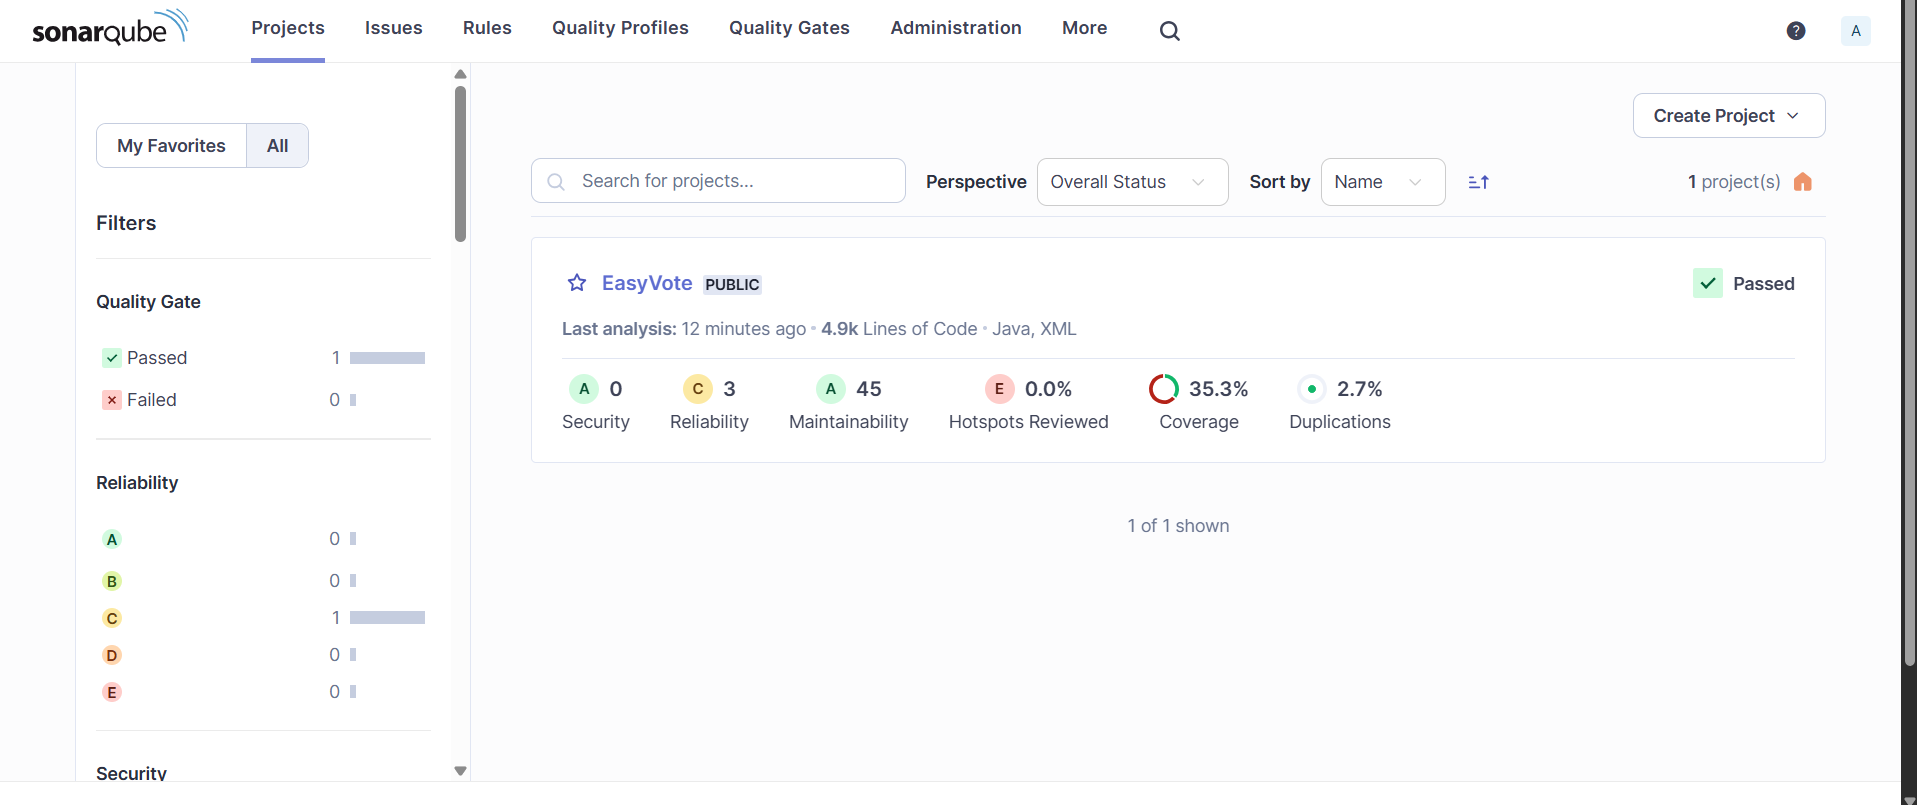
\includegraphics[width=0.95\textwidth]{images/sonarqube.png}
\caption{SonarQube --- projet EasyVote : Quality Gate réussi, 0 vulnérabilité, 3 bugs, 45 code smells, couverture 35,3\,\%, duplication 2,7\,\%}\label{fig:sonar}
\end{figure}

\subsection{Analyse statique outillée du frontend}
\begin{table}[H]
\centering
\caption{Résultats de l'analyse statique du frontend}
\small
\begin{tabularx}{\textwidth}{@{}p{1.1cm}p{2.2cm}p{5.4cm}X@{}}
\toprule
\rowcolor{evlight}\textbf{Réf.} & \textbf{Outil} & \textbf{Commande} & \textbf{Résultat}\\
\midrule
SA-01 & TypeScript & \texttt{npx tsc -b} & 0 erreur de typage\\
SA-02 & ESLint & \texttt{npx eslint .} & 64 erreurs, 5 avertissements (66 fichiers)\\
SA-03 & npm audit & \texttt{npm audit} & 35 vulnérabilités (1 critique, 26 hautes, 6 moyennes, 2 basses)\\
\bottomrule
\end{tabularx}
\end{table}

Parmi les erreurs ESLint : 30 \texttt{no-explicit-any} (typage affaibli) et surtout \textbf{4 \texttt{rules-of-hooks}} dans \texttt{ChatbotWidget.tsx} : un \texttt{return null} conditionnel (ligne 168) précède trois \texttt{useEffect} et un \texttt{useCallback}. Si la condition change entre deux rendus, React lève une erreur. Le composant n'étant monté que dans le tableau de bord, la défaillance ne se produit pas aujourd'hui : c'est un \textbf{défaut latent} (DEF-07) que seule l'analyse statique pouvait détecter.

% ------------------------------------------------------
\section{Techniques dynamiques boîte noire}

Ces techniques dérivent les cas de test des \textbf{spécifications} (cahier des charges), sans regarder le code. Elles sont automatisées en JUnit (dossier \nolinkurl{src/test/.../boitenoire}).

\subsection{Partition d'équivalence --- code OTP}
\textbf{Règle :} le code OTP contient exactement 6 chiffres. Un représentant par classe suffit.
\begin{table}[H]
\centering
\caption{Partitions d'équivalence du code OTP}
\small
\begin{tabular}{@{}llllc@{}}
\toprule
\rowcolor{evlight}\textbf{Réf.} & \textbf{Partition} & \textbf{Valeur} & \textbf{Attendu} & \textbf{Résultat}\\
\midrule
PE-01 & Valide (6 chiffres) & \texttt{123456} & Accepté & \ok\\
PE-02 & Invalide : longueur $\neq$ 6 & \texttt{12345} & Rejeté & \ok\\
PE-03 & Invalide : non numérique & \texttt{12AB56} & Rejeté (« uniquement des chiffres ») & \ok\\
\bottomrule
\end{tabular}
\end{table}

\subsection{Analyse des valeurs limites --- candidature}
\textbf{Règles :} slogan $\leq$ 200 caractères, photo $\leq$ 5\,Mo. On teste sur la limite et juste après.
\begin{table}[H]
\centering
\caption{Valeurs limites des champs de candidature}
\small
\begin{tabular}{@{}lllll@{}}
\toprule
\rowcolor{evlight}\textbf{Réf.} & \textbf{Champ} & \textbf{Valeur} & \textbf{Attendu} & \textbf{Résultat}\\
\midrule
VL-01 & Slogan & 200 caractères (limite) & Accepté & \ok\\
VL-02 & Slogan & 201 caractères (limite + 1) & Rejeté & \ok\\
VL-03 & Photo & 5 $\times$ 1024 $\times$ 1024 octets & Acceptée & \ko\ (DEF-01)\\
\bottomrule
\end{tabular}
\end{table}
VL-03 échoue avec le message « Fichier trop volumineux (max 5MB) » : le code compare la taille à 5\,000\,000 octets alors que 5\,Mo = 5\,242\,880 octets. Une valeur moyenne (2,5\,Mo) n'aurait jamais révélé ce défaut de frontière.

\subsection{Table de décision --- vote d'un étudiant}
Conditions : C1 = élection \texttt{VOTE\_ACTIVE} ; C2 = l'étudiant n'a pas déjà voté.
\begin{table}[H]
\centering
\caption{Table de décision du vote}
\small
\begin{tabular}{@{}lcclc@{}}
\toprule
\rowcolor{evlight}\textbf{Règle} & \textbf{C1} & \textbf{C2} & \textbf{Action attendue} & \textbf{Résultat}\\
\midrule
R1 & V & V & Vote enregistré + code de 10 caractères \texttt{[A-Z0-9]} & \ok\\
R2 & F & -- & Refus « Le vote n'est pas ouvert », aucun vote enregistré & \ok\\
R3 & V & F & Refus « Vous avez déjà voté », aucun vote enregistré & \ok\\
\bottomrule
\end{tabular}
\end{table}

\subsection{Test de transition d'état --- cycle de vie d'une élection}
États : \texttt{DRAFT} $\rightarrow$ \texttt{CAMPAIGN\_ACTIVE} $\rightarrow$ \texttt{VOTE\_ACTIVE} $\rightarrow$ \texttt{CLOSED}.
\begin{table}[H]
\centering
\caption{Transitions d'état de l'élection}
\small
\begin{tabular}{@{}lllc@{}}
\toprule
\rowcolor{evlight}\textbf{Réf.} & \textbf{Transition} & \textbf{Attendu} & \textbf{Résultat}\\
\midrule
ST-20 & DRAFT $\rightarrow$ CAMPAIGN\_ACTIVE & Acceptée & \ok\\
ST-21 & CAMPAIGN\_ACTIVE $\rightarrow$ VOTE\_ACTIVE & Acceptée & \ok\\
ST-23 & DRAFT $\rightarrow$ VOTE\_ACTIVE (saut d'état) & Rejetée, statut inchangé & \ok\\
\bottomrule
\end{tabular}
\end{table}

\subsection{Test des cas d'utilisation --- UC-03 « Voter »}
Le cas d'utilisation est joué de bout en bout au niveau système (section~\ref{sec:systeme}) et manuellement en acceptation (UAT-01).
\begin{table}[H]
\centering
\caption{Cas d'utilisation UC-03 : Voter}
\small
\begin{tabularx}{\textwidth}{@{}p{1cm}p{6.2cm}Xp{1.8cm}@{}}
\toprule
\rowcolor{evlight}\textbf{Étape} & \textbf{Action} & \textbf{Résultat attendu} & \textbf{Résultat}\\
\midrule
1 & Se connecter & JWT délivré & \ok\\
2 & Ouvrir l'élection \texttt{VOTE\_ACTIVE} & Liste des candidats validés & \ok\\
3 & Choisir un candidat et cocher « Je comprends que mon vote est définitif » & Confirmation demandée & \aex\\
4 & Confirmer & Vote enregistré + code de 10 caractères & \ok\\
5 & Consulter la participation & Statistiques visibles, choix non révélé & \ok\\
4b & Voter une 2\textsuperscript{e} fois (scénario alternatif) & Refus « déjà voté » & \ok\\
\bottomrule
\end{tabularx}
\end{table}

% ------------------------------------------------------
\section{Techniques dynamiques boîte blanche}

Ces techniques dérivent les tests de la \textbf{structure du code réel} (dossier \nolinkurl{src/test/.../boiteblanche}). La couverture obtenue est mesurée par JaCoCo.

\subsection{Couverture des instructions --- \texttt{hashToken()}}
\begin{lstlisting}[language=Java]
public String hashToken(String rawToken) {
    try {
        byte[] hash = MessageDigest.getInstance("SHA-256")
                .digest(rawToken.getBytes(StandardCharsets.UTF_8));
        StringBuilder sb = new StringBuilder();
        for (byte b : hash) sb.append(String.format("%02x", b));
        return sb.toString();
    } catch (NoSuchAlgorithmException e) {
        throw new RuntimeException("Erreur de hashage SHA-256 introuvable", e);
    }
}
\end{lstlisting}
\begin{table}[H]
\centering
\caption{Couverture des instructions de \texttt{hashToken()}}
\small
\begin{tabularx}{\textwidth}{@{}lp{3.3cm}Xc@{}}
\toprule
\rowcolor{evlight}\textbf{Réf.} & \textbf{Entrée} & \textbf{Attendu} & \textbf{Résultat}\\
\midrule
UT-01a & \texttt{"abc"} & \texttt{ba7816bf\ldots f20015ad} (vecteur officiel NIST) & \ok\\
UT-01b & jeton aléatoire & 64 caractères hexadécimaux, déterministe, $\neq$ jeton brut & \ok\\
UT-01c & deux générations & deux jetons bruts différents & \ok\\
\bottomrule
\end{tabularx}
\end{table}
Toutes les instructions atteignables sont couvertes. Le bloc \texttt{catch} est \textbf{inatteignable} (SHA-256 existe toujours dans la JVM) : 100\,\% des instructions est impossible ici, ce qui doit être justifié plutôt que forcé.

\subsection{Couverture des branches --- \texttt{generateTokensForElection()}}
\begin{lstlisting}[language=Java]
Election election = electionRepository.findById(electionId).orElseThrow(...); // B1
if (voteTokenRepository.existsByElectionId(electionId)) { return; }          // B2
for (User user : userRepository.findByIsVerifiedTrue()) {                     // B3
    String tokenHash = hashToken(generateRawToken());
    voteTokenRepository.save(VoteToken.builder()...tokenHash(tokenHash)...build());
}
\end{lstlisting}
\begin{table}[H]
\centering
\caption{Couverture des branches de la génération des jetons}
\small
\begin{tabularx}{\textwidth}{@{}lp{3.2cm}p{3.4cm}Xc@{}}
\toprule
\rowcolor{evlight}\textbf{Réf.} & \textbf{Branche} & \textbf{Données} & \textbf{Attendu} & \textbf{Résultat}\\
\midrule
B1 & Élection introuvable & id inexistant & \texttt{ResourceNotFoundException} & \ok\\
B2 & Jetons déjà générés & \texttt{existsByElectionId} = vrai & aucun \texttt{save()} (idempotence) & \ok\\
B3 & Génération & 3 étudiants vérifiés & 3 jetons, hash de 64 caractères, tous distincts & \ok\\
\bottomrule
\end{tabularx}
\end{table}
JaCoCo confirme \textbf{100\,\% des branches} de \texttt{VoteTokenService}.

\subsection{Couverture des décisions --- \texttt{validateDates()}}
Trois décisions :
\begin{itemize}
  \item D1 : \texttt{!campaignStart.isBefore(campaignEnd)}
  \item D2 : \texttt{campaignEnd.isAfter(voteStart)}
  \item D3 : \texttt{!voteStart.isBefore(voteEnd)}
\end{itemize}
\begin{table}[H]
\centering
\caption{Couverture des décisions de la validation des dates}
\small
\begin{tabular}{@{}lccclc@{}}
\toprule
\rowcolor{evlight}\textbf{Réf.} & \textbf{D1} & \textbf{D2} & \textbf{D3} & \textbf{Résultat attendu} & \textbf{Résultat}\\
\midrule
DC-01 & F & F & F & Élection créée en DRAFT & \ok\\
DC-02 & V & -- & -- & Rejet « début de campagne » & \ok\\
DC-03 & F & F & V & Rejet « début de vote » & \ok\\
\bottomrule
\end{tabular}
\end{table}
D2 n'est évaluée qu'à FAUX : un quatrième cas serait nécessaire pour 100\,\% de couverture des décisions (limite assumée de l'échantillon).

\subsection{Complexité cyclomatique --- \texttt{castVote()}}
La méthode \texttt{VoteService.castVote()} contient 11 points de décision : utilisateur absent, compte non vérifié, élection absente, candidat absent, candidat d'une autre élection, candidat non validé, statut $\neq$ \texttt{VOTE\_ACTIVE}, fin de vote (2 conditions), jeton absent, jeton déjà utilisé.
\begin{center}\textbf{V(G) = nombre de décisions + 1 = 11 + 1 = 12}\end{center}
Le seuil habituel de 10 est dépassé (UT-07 en échec) : la méthode devrait être découpée. Les chemins indépendants sont répartis entre la table de décision, le MC/DC et les trois chemins suivants :
\begin{table}[H]
\centering
\caption{Chemins indépendants de \texttt{castVote()}}
\small
\begin{tabularx}{\textwidth}{@{}lp{4.4cm}Xc@{}}
\toprule
\rowcolor{evlight}\textbf{Réf.} & \textbf{Chemin} & \textbf{Attendu} & \textbf{Résultat}\\
\midrule
CC-1 & sortie à la décision 2 & compte non vérifié : \texttt{ForbiddenException} & \ok\\
CC-2 & sortie à la décision 5 & candidat d'une autre élection : refus & \ok\\
CC-3 & jeton absent $\rightarrow$ généré à la volée & vote enregistré avec un hash de 64 caractères ; l'entité \texttt{Vote} n'a aucun champ \texttt{User} & \ok\\
\bottomrule
\end{tabularx}
\end{table}

\subsection{Couverture MC/DC --- fin de la période de vote}
\begin{lstlisting}[language=Java]
if (election.getVoteEnd() != null && now.isAfter(election.getVoteEnd()))   // condition A, condition B
    throw new BusinessException("La période de vote est terminée");
\end{lstlisting}
Pour $n = 2$ conditions, MC/DC exige $n + 1 = 3$ tests où chaque condition change seule la décision.
\begin{table}[H]
\centering
\caption{Couverture MC/DC de la condition de fin de vote}
\small
\begin{tabular}{@{}lccllc@{}}
\toprule
\rowcolor{evlight}\textbf{Test} & \textbf{A} & \textbf{B} & \textbf{Décision} & \textbf{Paire démontrée} & \textbf{Résultat}\\
\midrule
T1 & V & V & V (vote refusé) & --- & \ok\\
T2 & V & F & F (vote accepté) & (T1, T2) : B influe seul & \ok\\
T3 & F & -- & F (vote accepté) & (T1, T3) : A influe seul & \ok\\
\bottomrule
\end{tabular}
\end{table}

\subsection{Couverture mesurée par JaCoCo}
\begin{table}[H]
\centering
\caption{Couverture de code mesurée (JaCoCo)}
\small
\begin{tabular}{@{}lcc@{}}
\toprule
\rowcolor{evlight}\textbf{Classe} & \textbf{Lignes} & \textbf{Branches}\\
\midrule
VoteTokenService & 84,2\,\% & 100\,\%\\
VoteService & 66,3\,\% & 60,7\,\%\\
VoteAnalyticsService & 57,4\,\% & 35,0\,\%\\
ElectionService & 56,0\,\% & 42,2\,\%\\
JwtUtil & 66,0\,\% & 50,0\,\%\\
ChatbotRulesService & 34,1\,\% & 30,3\,\%\\
\midrule
Projet complet & 38,0\,\% & 25,3\,\%\\
\bottomrule
\end{tabular}
\end{table}
La couverture globale est faible car seuls les modules critiques ont été ciblés ; elle est élevée là où le risque est le plus fort (jetons et vote).

\begin{figure}[H]
\centering
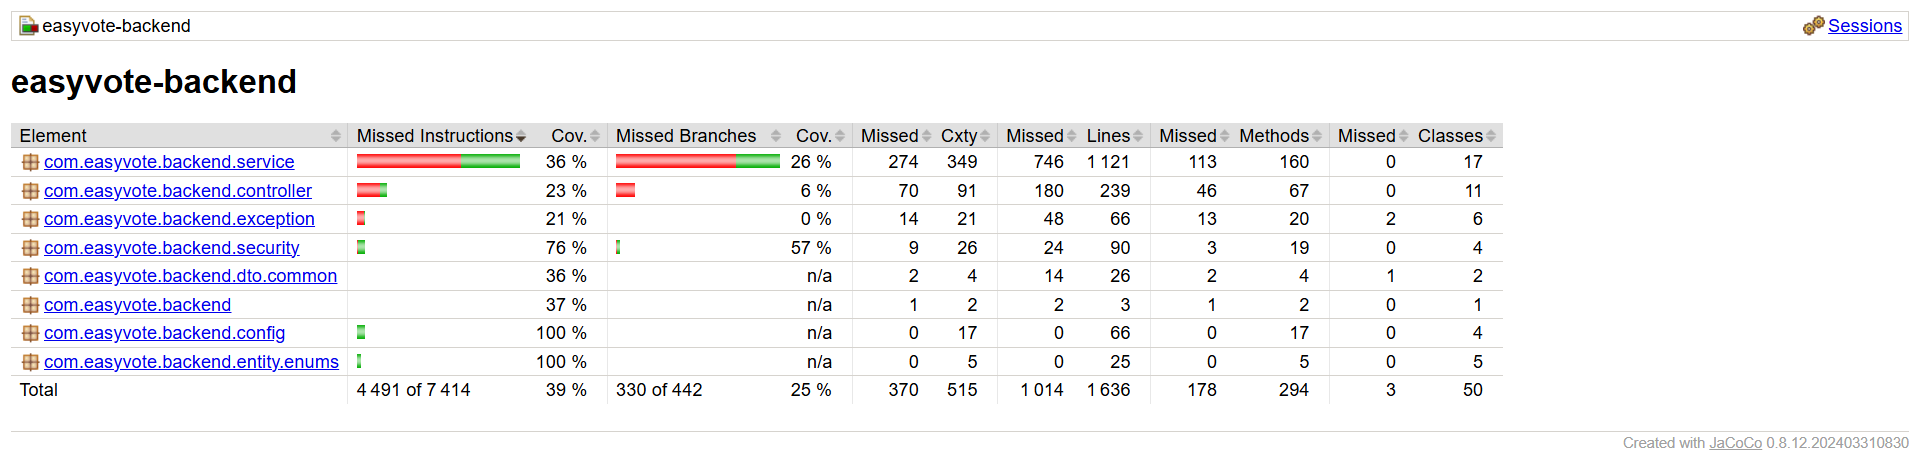
\includegraphics[width=\textwidth]{images/jacoco.png}
\caption{Rapport JaCoCo --- couverture par paquet : 39\,\% des instructions et 25\,\% des branches (1\,636 lignes, 38\,\% couvertes)}\label{fig:jacoco}
\end{figure}

% ------------------------------------------------------
\section{Tests unitaires : chatbot et non-régression}
\begin{table}[H]
\centering
\caption{Tests unitaires du chatbot EasyBot et de non-régression}
\small
\begin{tabularx}{\textwidth}{@{}lp{2.4cm}Xc@{}}
\toprule
\rowcolor{evlight}\textbf{Réf.} & \textbf{Type} & \textbf{Vérification} & \textbf{Résultat}\\
\midrule
UT-01 (chatbot) & Fonctionnel & « Bonjour » $\rightarrow$ message de bienvenue & \ok\\
UT-06 & Non fonctionnel & réponse de la couche règles en moins de 50\,ms & \ok\\
UT-M01 & Régression & jeu de 10 votes de référence (5, 3 et 2 voix) sur 20 électeurs : classement, pourcentages (50, 30 et 20\,\%) et participation (50\,\%) inchangés & \ok\\
\bottomrule
\end{tabularx}
\end{table}
UT-M01 appelle \texttt{VoteAnalyticsService.getResults()} avec des dépôts simulés ; les candidats sont fournis dans le désordre pour vérifier aussi le tri. Les valeurs attendues sont figées : après un refactoring, le résultat doit rester identique. Dans le script \texttt{lancer-tests.ps1}, le test chatbot « Bonjour » porte l'identifiant UT-01, à ne pas confondre avec UT-01a à UT-01c (\texttt{hashToken()}) du plan.

Le test UT-CB3 (« Comment devenir candidat ? »), qui avait révélé le défaut DEF-04, a été retiré de la suite automatisée. Réponse obtenue à l'époque : « Il n'y a pas d'élection en cours, donc pas de liste de candidats. » Les règles étant évaluées dans l'ordre, la règle « candidat » est déclenchée avant la règle « devenir candidat ». \textbf{Le défaut n'est pas corrigé} : il reste ouvert dans la liste des défauts.

% ------------------------------------------------------
\section{Tests d'intégration et tests d'API}

\subsection{Tests d'intégration automatisés (JUnit + MockMvc + H2)}
L'application Spring démarre réellement (contrôleurs, filtre JWT, services, JPA) sur une base H2 en mémoire ; seul l'envoi d'email est simulé.
\begin{table}[H]
\centering
\caption{Tests d'intégration exécutés}
\small
\begin{tabularx}{\textwidth}{@{}lp{4.4cm}Xp{1.9cm}@{}}
\toprule
\rowcolor{evlight}\textbf{Réf.} & \textbf{Scénario} & \textbf{Vérifications} & \textbf{Résultat}\\
\midrule
IT-01 & POST \nolinkurl{/api/auth/register} & HTTP 201 ; compte STUDENT non vérifié ; mot de passe haché BCrypt ; OTP à 6 chiffres envoyé & \ok\\
IT-09 & GET \nolinkurl{/api/admin/users} & sans jeton $\rightarrow$ 401 ; jeton STUDENT $\rightarrow$ 403 & \ok\\
IT-04 & POST \nolinkurl{/api/elections/{id}/vote} & HTTP 201 et code de 10 caractères ; pas de colonne \texttt{user\_id} ; aucune jointure ne relie un électeur à son vote & \ko\ (DEF-00)\\
IT-07 & GET \nolinkurl{/api/elections} & 5 élections ; 20 appels successifs après un appel de chauffe ; temps de réponse moyen $\leq$ 200\,ms & \ok\\
\bottomrule
\end{tabularx}
\end{table}

\subsection{Tests d'API avec Postman}
Une collection Postman (\texttt{tests/postman/EasyVote.postman\_collection.json}) automatise les vérifications sur l'API réelle. Le jeton obtenu par PM-01 est stocké dans une variable et réutilisé par PM-03. La collection est exécutable dans Postman (\textit{Run collection}) ou en ligne de commande avec Newman.
\begin{table}[H]
\centering
\caption{Tests Postman}
\small
\begin{tabularx}{\textwidth}{@{}lp{4.2cm}p{2cm}Xc@{}}
\toprule
\rowcolor{evlight}\textbf{Réf.} & \textbf{Requête} & \textbf{Type} & \textbf{Assertions} & \textbf{Résultat}\\
\midrule
PM-01 & POST \nolinkurl{/api/auth/login} & Fonctionnel & statut 200 ; jeton renvoyé ; rôle ADMIN & \ok\\
PM-03 & GET \nolinkurl{/api/auth/me} (Bearer) & Fonctionnel & statut 200 ; profil du jeton ; mot de passe jamais renvoyé & \ok\\
PM-02 & GET \nolinkurl{/api/admin/users} sans jeton & Non fonct. (sécurité) & statut 401 ; message « Authentification requise » ; réponse $<$ 200\,ms & \ok\\
\bottomrule
\end{tabularx}
\end{table}
\begin{lstlisting}[language=Java,caption={Script de test Postman de PM-01}]
pm.test("Statut HTTP 200", function () {
    pm.response.to.have.status(200);
});
const json = pm.response.json();
pm.test("Le rôle de l'utilisateur est ADMIN", function () {
    pm.expect(json.data.user.role).to.eql("ADMIN");
});
pm.collectionVariables.set("token", json.data.accessToken);  // réutilisé par PM-03
\end{lstlisting}
\begin{lstlisting}[caption={Exécution de la collection avec Newman}]
-> PM-01 Connexion administrateur (fonctionnel)
  POST http://localhost:8082/api/auth/login [200 OK, 90ms]
  v  Statut HTTP 200
  v  Un jeton JWT est renvoyé
  v  Le rôle de l'utilisateur est ADMIN
-> PM-03 Profil connecté /auth/me avec le jeton (fonctionnel)
  GET http://localhost:8082/api/auth/me [200 OK, 9ms]
  v  Statut HTTP 200
  v  Le profil renvoyé est celui du jeton (ahmed@test.com, ADMIN)
  v  Le mot de passe n'est jamais renvoyé
-> PM-02 Route admin protégée sans jeton (non fonctionnel : sécurité)
  GET http://localhost:8082/api/admin/users [401 Unauthorized, 4ms]
  v  Accès refusé : statut HTTP 401
  v  Message « Authentification requise »
  v  Réponse en moins de 200 ms (CDC 5.1)
assertions : 9 exécutées, 0 en échec
\end{lstlisting}
\begin{figure}[H]
\centering
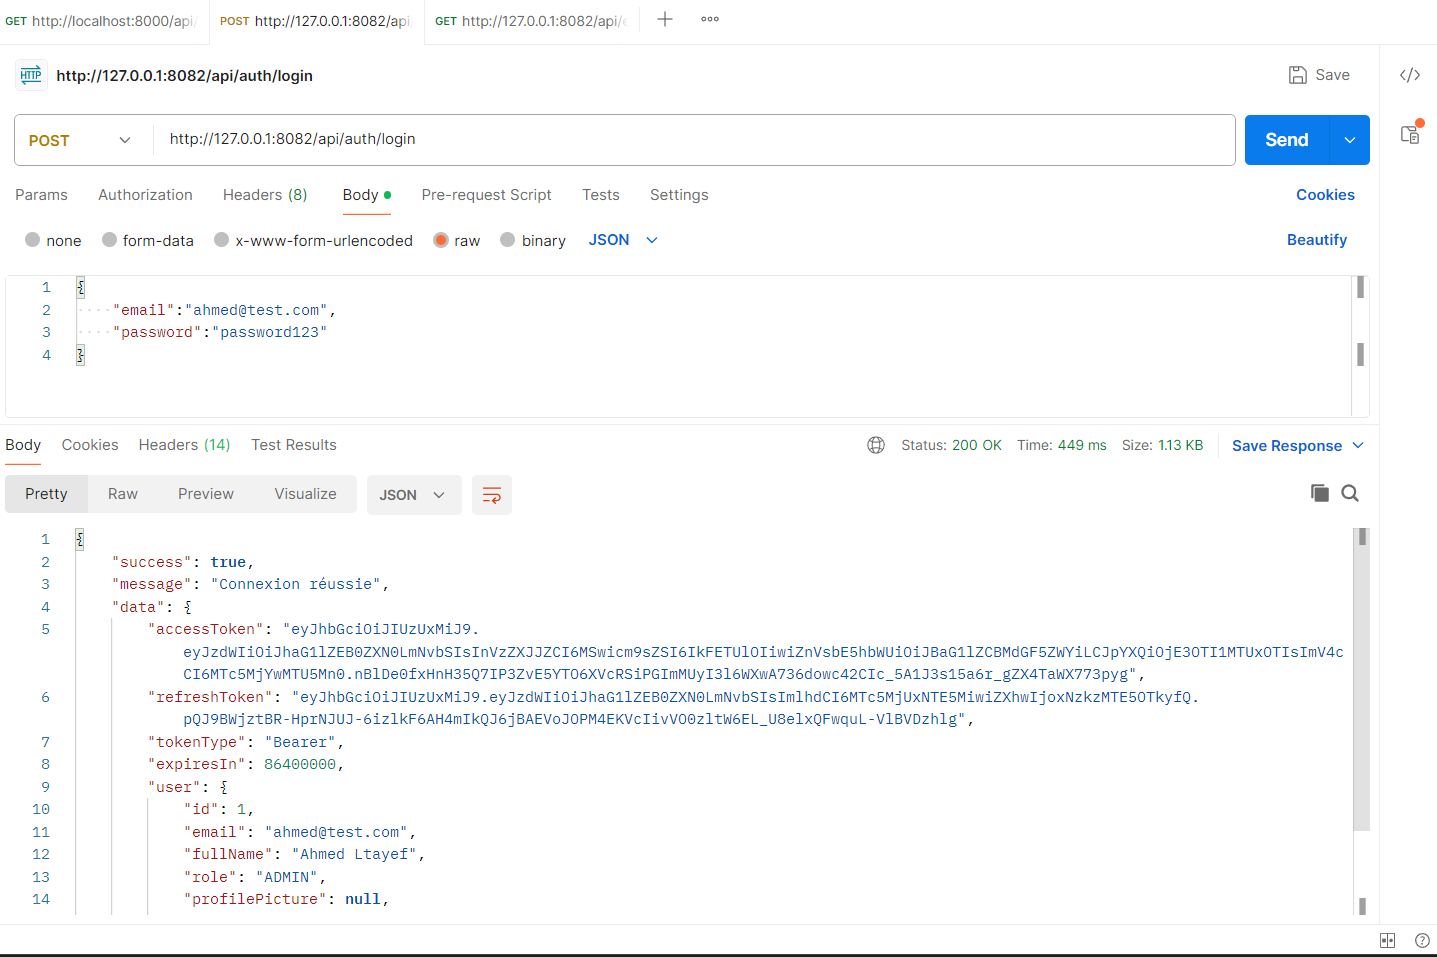
\includegraphics[width=0.85\textwidth]{images/postman-login.png}
\caption{Postman --- PM-01 : \texttt{POST /api/auth/login} avec le compte administrateur, 200 OK ; le jeton d'accès, le jeton de rafraîchissement et \texttt{expiresIn} (86\,400\,000 ms, soit 24\,h) sont renvoyés}\label{fig:pm-login}
\end{figure}

\begin{figure}[H]
\centering
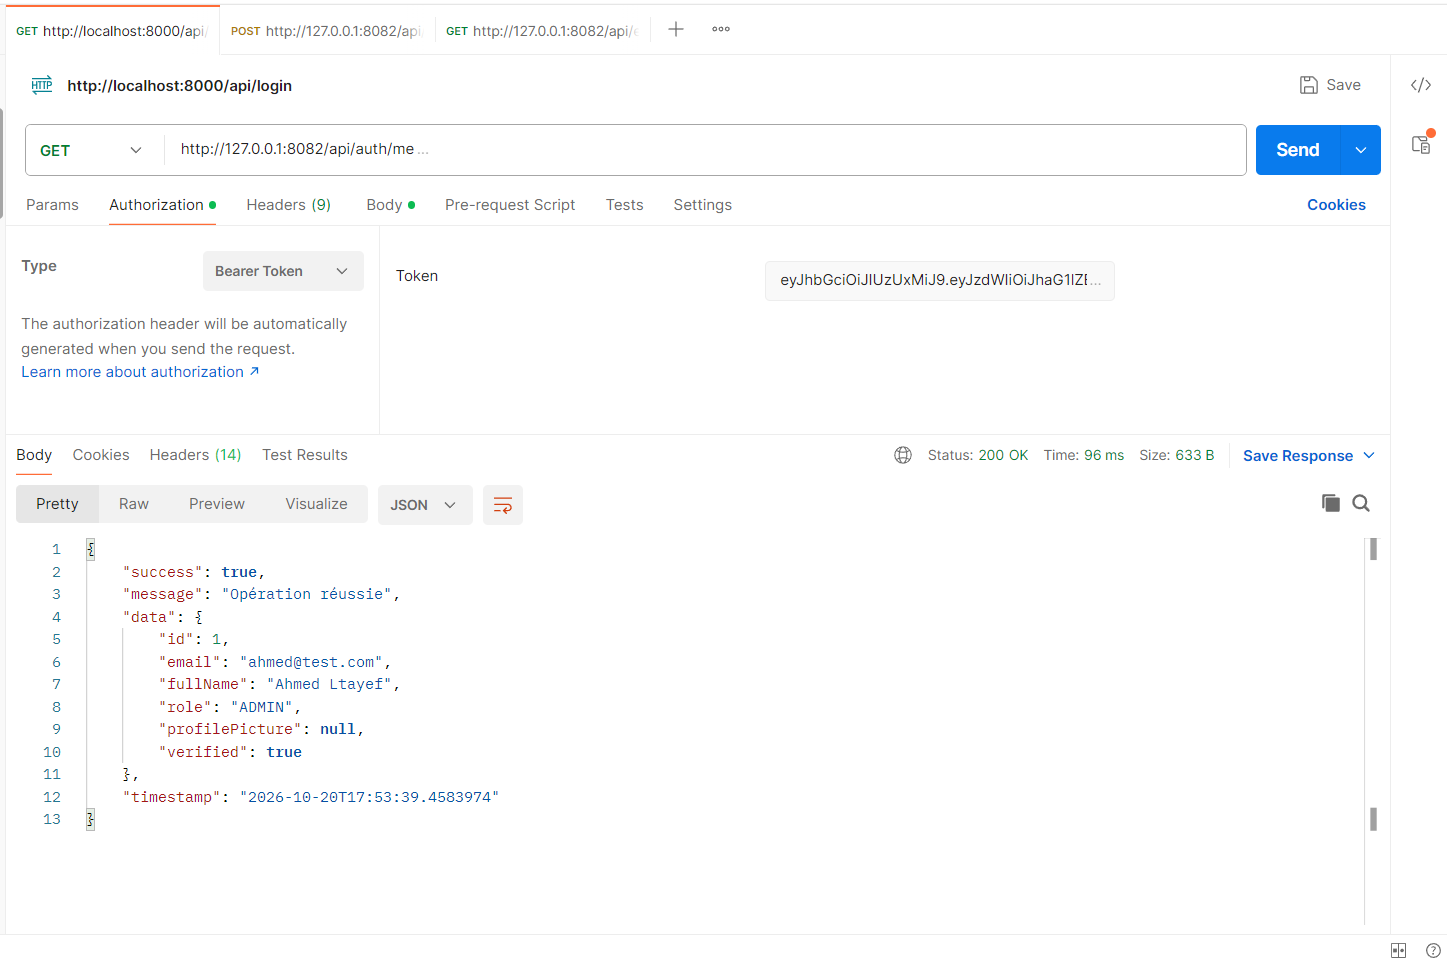
\includegraphics[width=0.85\textwidth]{images/postman-auth-me.png}
\caption{Postman --- PM-03 : \texttt{GET /api/auth/me} avec le jeton en \textit{Bearer Token}, 200 OK en 96\,ms ; le profil est celui du jeton et le mot de passe n'est pas renvoyé}\label{fig:pm-me}
\end{figure}

\begin{figure}[H]
\centering
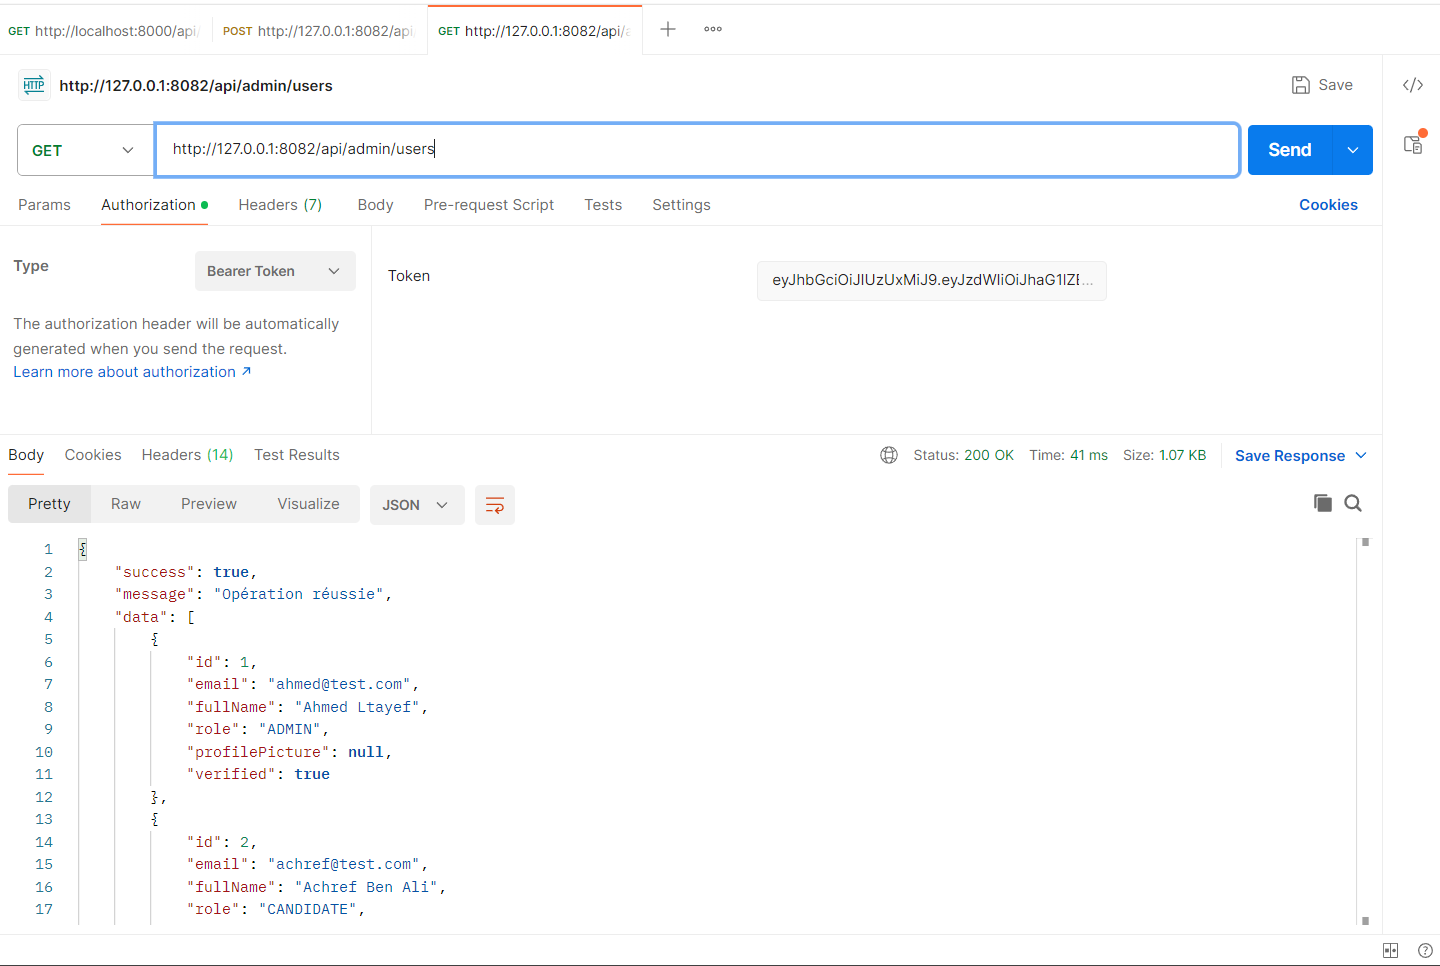
\includegraphics[width=0.85\textwidth]{images/postman-admin-users.png}
\caption{Postman --- \texttt{GET /api/admin/users} avec le jeton ADMIN, 200 OK en 41\,ms : la contrepartie de PM-02, qui renvoie 401 sans jeton}\label{fig:pm-admin}
\end{figure}

\subsection{Vérification manuelle du JWT avec jwt.io (JWT-01)}
Le jeton renvoyé par \texttt{/api/auth/login} a été décodé sur \url{https://jwt.io} pour vérifier son contenu par rapport au cahier des charges (§4.4.1 : access token valide 1\,h).
\begin{lstlisting}[caption={Contenu décodé d'un access token EasyVote}]
HEADER  : { "alg": "HS512" }
PAYLOAD : { "sub": "ahmed@test.com", "userId": 1, "role": "ADMIN",
            "fullName": "Ahmed Ltayef", "iat": 1792444682, "exp": 1792531082 }
exp - iat = 86400 s = 24 h
\end{lstlisting}
\begin{itemize}
  \item \textbf{Conforme :} l'algorithme de signature (HS512), l'identité (\texttt{sub}, \texttt{userId}) et le rôle sont présents et cohérents avec \texttt{/auth/me}.
  \item \textbf{Non conforme :} la durée de validité est de \textbf{24\,h} au lieu de 1\,h. Le défaut DEF-06, trouvé en revue (RV-01), est ainsi \textbf{confirmé dynamiquement}.
  \item \textbf{Observation :} le payload d'un JWT est seulement encodé (Base64), pas chiffré : l'email et le nom complet sont lisibles par quiconque possède le jeton.
\end{itemize}
\begin{figure}[H]
\centering
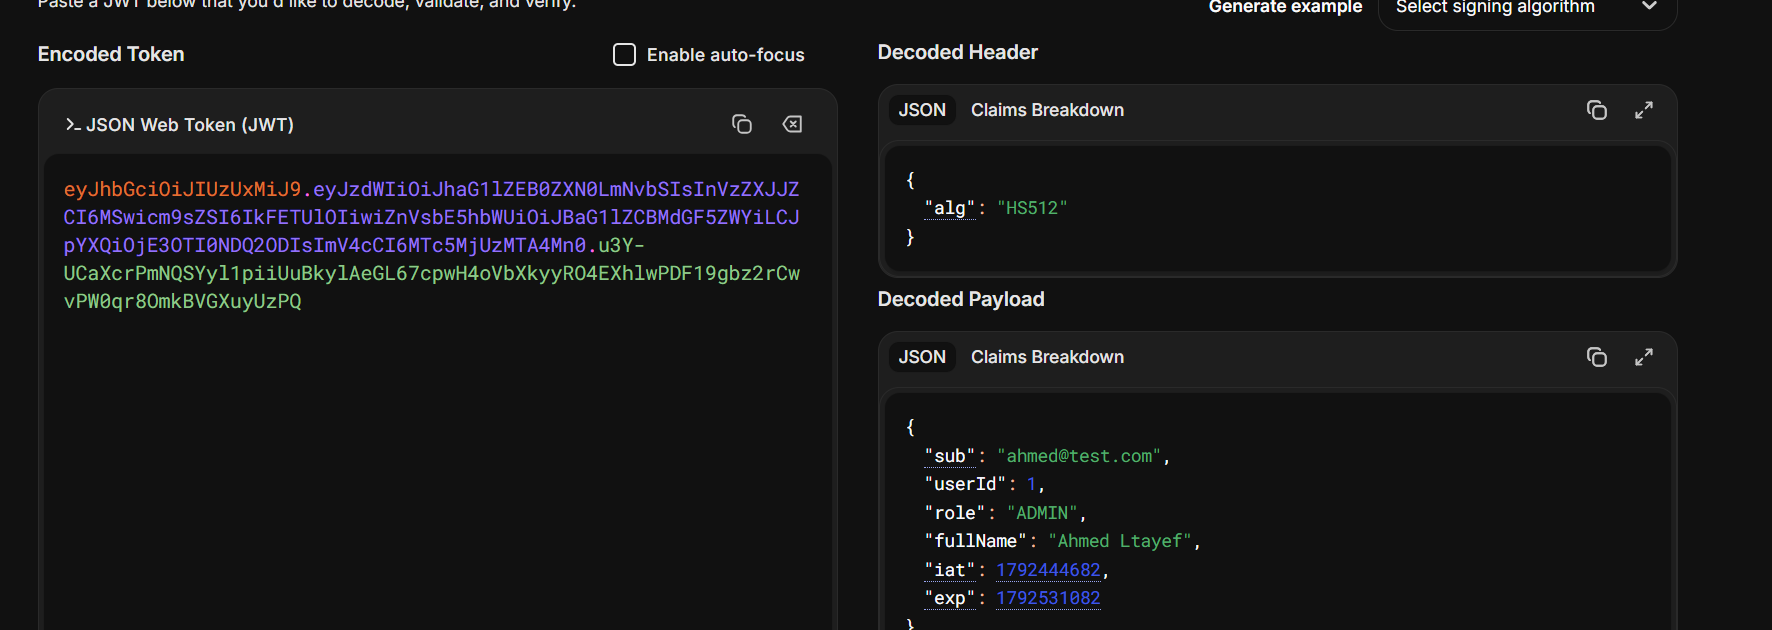
\includegraphics[width=\textwidth]{images/jwt-io.png}
\caption{jwt.io --- access token décodé : algorithme HS512, rôle ADMIN, \texttt{iat} = 1792444682 et \texttt{exp} = 1792531082 (écart de 86\,400 s, soit 24\,h)}\label{fig:jwt}
\end{figure}

% ------------------------------------------------------
\section{Tests système de bout en bout}\label{sec:systeme}
Le script \texttt{tests/system-tests.mjs} pilote l'application complète (backend + MariaDB) comme le ferait l'interface. Il joue le scénario de démonstration du cahier des charges (§7.3) et le cas d'utilisation UC-03.
\begin{lstlisting}[caption={Exécution des tests système}]
ST-01 Scénario complet : création -> candidature -> validation -> vote -> résultats
  [OK] ST-01.1 l'admin crée une élection (DRAFT)
  [OK] ST-01.2 ouverture de la campagne
  [OK] ST-01.3 un étudiant postule (PENDING)
  [OK] ST-01.4 l'admin valide la candidature
  [OK] ST-01.5 ouverture du vote + génération des jetons
  [OK] ST-01.6 l'étudiant vote -> code de confirmation « UNVEB634QL »
ST-02 Interdiction du double vote
  [OK] ST-02 le 2e vote est refusé avec un message clair
ST-03 Transparence : participation pendant le vote, détails après clôture
  [OK] ST-03.1 pendant le vote, l'étudiant ne voit PAS les résultats détaillés
  [OK] ST-03.2 pendant le vote, l'étudiant voit la participation
  [OK] ST-03.3 après clôture, résultats détaillés publiés (rang 1 = 100 %)
  [OK] ST-05 export du rapport PDF officiel
ST-NF Performance
  [OK] ST-NF GET /elections : moyenne 61.1 ms sur 20 appels (< 200 ms)
Bilan : 12 vérifications réussies, 0 en échec.
\end{lstlisting}
Une 13\textsuperscript{e} vérification, \textbf{REG-002} (non-régression du calcul des résultats : après la clôture, classement, votes, pourcentages et participation sont identiques entre deux lectures de \texttt{/results}), a été ajoutée au script après cette exécution. Elle est \aex\ : elle demande le backend et les comptes de test chargés.

% ------------------------------------------------------
\section{Tests de charge et de performance avec JMeter}
Apache JMeter 5.6.3 exécute le plan \texttt{tests/jmeter/EasyVote-charge.jmx} (ST-08). Chaque utilisateur virtuel se connecte une fois (\texttt{POST /api/auth/login}, extraction du jeton JWT), puis consulte en boucle la liste des élections et les statistiques de participation, avec une pause de 300\,ms. Deux assertions sont appliquées à chaque requête : code HTTP 200 et temps de réponse inférieur à \textbf{200\,ms} (CDC §5.1). Le test se lance avec \texttt{tests/jmeter-charge.ps1 -Users N} et produit un rapport HTML.

\begin{table}[H]
\centering
\caption{Résultats JMeter selon le nombre d'utilisateurs simultanés}
\small
\begin{tabular}{@{}lrrrrr@{}}
\toprule
\rowcolor{evlight}\textbf{Scénario} & \textbf{Requêtes} & \textbf{HTTP 200} & \textbf{Plus de 200 ms} & \textbf{Moyenne} & \textbf{90e centile}\\
\midrule
50 utilisateurs $\times$ 10 boucles & 1\,050 & 100\,\% & 0\,\% & 12 ms & 14 ms\\
200 utilisateurs $\times$ 5 boucles & 2\,200 & 100\,\% & 0\,\% & 14 ms & 20 ms\\
500 utilisateurs $\times$ 5 boucles & 5\,500 & 100\,\% & 51,8\,\% & 486 ms & 1\,172 ms\\
\bottomrule
\end{tabular}
\end{table}

\begin{itemize}
  \item \textbf{Fonctionnel sous charge :} aucune erreur HTTP, même à 500 utilisateurs (5\,500 réponses 200).
  \item \textbf{Performance :} l'exigence de 200\,ms est respectée jusqu'à 200 utilisateurs, mais \textbf{pas à 500} : 2\,847 requêtes dépassent 200\,ms, et la connexion (hachage BCrypt) monte à 593\,ms en moyenne. C'est la non-conformité \textbf{DEF-08}.
  \item \textbf{Limite de la mesure :} le test a été exécuté sur un poste de développement, avec JMeter, le backend et la base sur la même machine. Le résultat est à confirmer sur un serveur dédié avant toute conclusion définitive.
\end{itemize}

\begin{figure}[H]
\centering
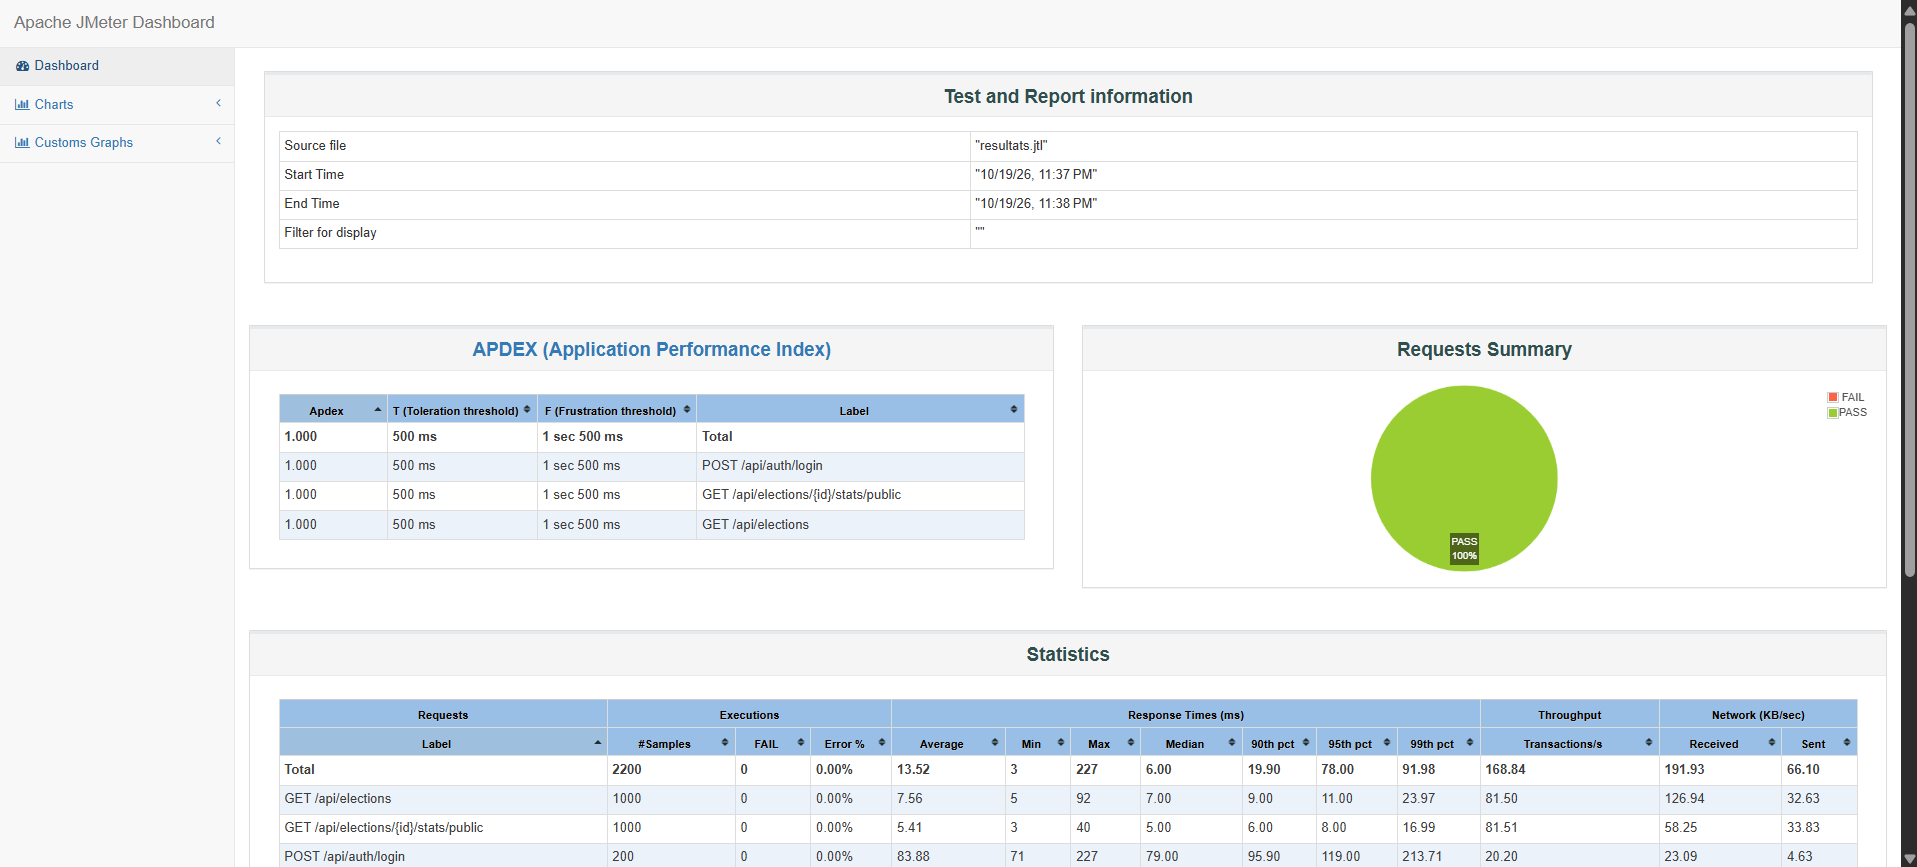
\includegraphics[width=\textwidth]{images/jmeter.png}
\caption{Rapport JMeter --- scénario à 200 utilisateurs : 2\,200 requêtes, 0 erreur, temps moyen 13,5\,ms, 90\textsuperscript{e} centile 19,9\,ms}\label{fig:jmeter}
\end{figure}

% ------------------------------------------------------
\section{Tests manuels}

\subsection{Vérification SQL de l'anonymat (SQL-01)}\label{sec:anonymat}
Le plan initial vérifiait seulement l'absence de colonne \texttt{user\_id} dans la table \texttt{votes}. Ce test passe, mais il ne prouve pas l'exigence du cahier des charges (§4.4.2) : « aucune requête SQL ne peut établir de lien entre un utilisateur et son vote ». Or la table \texttt{votes} stocke le même \texttt{token\_hash} que la table \texttt{vote\_tokens}, qui contient \texttt{user\_id}. Sur la base réelle :
\begin{lstlisting}[language=SQL,caption={Requête SQL de ré-identification d'un vote}]
SELECT u.email AS electeur, cu.full_name AS a_vote_pour
FROM votes v
JOIN vote_tokens t ON t.token_hash = v.token_hash
JOIN users u       ON u.id = t.user_id
JOIN candidates c  ON c.id = v.candidate_id
JOIN users cu      ON cu.id = c.user_id;

electeur         a_vote_pour
talel@test.com   Achref Ben Ali
\end{lstlisting}
N'importe quel administrateur ayant accès à la base peut donc savoir pour qui chaque étudiant a voté : c'est le \textbf{défaut critique DEF-00}. Le test d'intégration IT-04 a été renforcé avec cette jointure et échoue désormais, comme il le doit. \textbf{Leçon :} un test doit vérifier l'exigence, pas l'implémentation supposée.

\textit{Piste de correction :} ne stocker dans \texttt{votes} aucune valeur reliable au jeton (ou un hash salé avec un secret différent), et ne conserver dans \texttt{vote\_tokens} que l'indicateur \og déjà voté \fg.

\subsection{Tests exploratoires}\label{sec:explo}
Guidés par la revue technique, ces tests vérifient trois règles du cahier des charges sur l'application en fonctionnement (rejoués par \texttt{tests/exploratoire.mjs}).
\begin{table}[H]
\centering
\caption{Tests exploratoires}
\small
\begin{tabularx}{\textwidth}{@{}lXp{3.6cm}p{3.2cm}@{}}
\toprule
\rowcolor{evlight}\textbf{Réf.} & \textbf{Action} & \textbf{Attendu (CDC)} & \textbf{Obtenu}\\
\midrule
EX-1 & Postuler à une élection encore en DRAFT & Refus (§3.1.2) & HTTP 201 : \ko\ (DEF-03)\\
EX-2 & Lire \texttt{/api/auth/me} avec une candidature PENDING & Rôle STUDENT & CANDIDATE : \ko\ (DEF-02)\\
EX-3 & Voter avec le compte administrateur & Refus (§6.1) & Vote enregistré : \ko\ (DEF-05)\\
\bottomrule
\end{tabularx}
\end{table}

\subsection{Tests d'acceptation automatisés}\label{sec:uat-auto}
Un cas automatisable par type de test a été écrit dans \texttt{AcceptationTest} (JUnit, MockMvc, H2) : le scénario est joué comme le ferait l'utilisateur, par l'API, avec une connexion réelle et non un jeton fabriqué.
\begin{table}[H]
\centering
\caption{Tests d'acceptation automatisés}
\small
\begin{tabularx}{\textwidth}{@{}lp{1.9cm}Xc@{}}
\toprule
\rowcolor{evlight}\textbf{Réf.} & \textbf{Type} & \textbf{Vérification} & \textbf{Résultat}\\
\midrule
UAT-01 & Fonct. & étudiant : connexion $\rightarrow$ consultation des élections $\rightarrow$ vote avec code de confirmation, sans blocage & \ok\\
UAT-06 & Non-fonct. & le PDF des résultats est un vrai document (en-tête \texttt{\%PDF}, taille $>$ 1\,000 octets) ; sa clarté reste à juger par un lecteur & \ok\\
UAT-07 & Struct. & les trois rôles accèdent à \texttt{/auth/me} et \texttt{/elections} ; \texttt{/admin/users} répond 200 à l'ADMIN et 403 au STUDENT et au CANDIDATE & \ok\\
UAT-M03 & Régr. & création et pilotage d'une élection : 401 pour un anonyme, 403 pour un étudiant, autorisé pour l'ADMIN & \ok\\
\bottomrule
\end{tabularx}
\end{table}

\subsection{Tests d'acceptation manuels (UAT)}
Les autres tests d'acceptation sont exécutés manuellement dans le navigateur, chaque membre jouant un rôle et notant la facilité d'utilisation de 1 à 5.
\begin{table}[H]
\centering
\caption{Exécution des tests d'acceptation}
\small
\begin{tabularx}{\textwidth}{@{}lp{2.2cm}Xp{1.8cm}p{1.4cm}@{}}
\toprule
\rowcolor{evlight}\textbf{Réf.} & \textbf{Testeur} & \textbf{Scénario} & \textbf{Résultat} & \textbf{Note /5}\\
\midrule
UAT-01 & Rawen (étudiant) & connexion $\rightarrow$ programme $\rightarrow$ vote avec confirmation $\rightarrow$ code & [à compléter] & [ \_ ]\\
UAT-02 & Issra (candidat) & Ma campagne $\rightarrow$ programme $\rightarrow$ annonce $\rightarrow$ réponse & [à compléter] & [ \_ ]\\
UAT-03 & Talel (admin) & création $\rightarrow$ validation $\rightarrow$ vote $\rightarrow$ clôture $\rightarrow$ PDF & [à compléter] & [ \_ ]\\
\bottomrule
\end{tabularx}
\end{table}

\subsection{Test de maintenance : sauvegarde et restauration}
Le script \texttt{tests/maintenance-sauvegarde.ps1} sauvegarde la base (\texttt{mysqldump}), la restaure dans une copie et compare le contenu table par table, sans toucher à la base réelle.
\begin{lstlisting}[caption={Exécution du test de maintenance}]
[OK]    MT-01 sauvegarde creee : tests\sauvegarde.sql
        users        original =   5   restauree =   5
        elections    original =   3   restauree =   3
        candidates   original =   3   restauree =   3
        votes        original =   3   restauree =   3
        vote_tokens  original =   7   restauree =   7
[OK]    MT-02 donnees restaurees a l'identique
\end{lstlisting}

\subsection{Tests liés aux changements : confirmation et régression}
La suite automatisée est \textbf{entièrement rejouable}. Après correction d'un défaut (par exemple DEF-01 : remplacer \texttt{5\_000\_000} par \texttt{5 * 1024 * 1024}), on exécute :
\begin{itemize}
  \item un \textbf{test de confirmation} : le test VL-03 (\texttt{lancer-tests.ps1 VL-03}) doit passer au vert ;
  \item un \textbf{test de régression} : toute la suite (\texttt{lancer-tests.ps1}, puis \texttt{system-tests.mjs}) est relancée et tous les autres tests doivent rester verts.
\end{itemize}

% ------------------------------------------------------
\section{Tests manuels et automatisés : synthèse}
\begin{table}[H]
\centering
\caption{Répartition des tests exécutés par technique et par mode}
\small
\begin{tabularx}{\textwidth}{@{}p{3.6cm}XX@{}}
\toprule
\rowcolor{evlight}\textbf{Technique} & \textbf{Manuel} & \textbf{Automatisé}\\
\midrule
Statique & Revue technique (RV-01..06), tri des alertes SonarQube & SonarQube, ESLint, tsc, npm audit (SA-01..03)\\
Boîte noire & UAT-01..03, cas d'utilisation UC-03 & PE, VL, R, ST-20/21/23 (12 tests JUnit)\\
Boîte blanche & Calcul de V(G) & UT-01, B, DC, CC, T (15 tests JUnit) + JaCoCo\\
Intégration / API & jwt.io (JWT-01) & IT-01/04/07/09 (JUnit), PM-01..03 (Postman)\\
Système & SQL-01, exploratoires EX-1..3 & \texttt{system-tests.mjs} (12 vérifications), JMeter (ST-08)\\
Unitaire / régression & --- & UT-01 (chatbot), UT-06, UT-M01 (3 tests JUnit)\\
Acceptation & UAT-01..03 en navigateur & UAT-01, 06, 07, M03 (4 tests JUnit)\\
Maintenance & --- & MT-01, MT-02\\
\bottomrule
\end{tabularx}
\end{table}

% ------------------------------------------------------
\section{Bilan de l'exécution}

\begin{table}[H]
\centering
\caption{Bilan chiffré de l'exécution}
\small
\begin{tabular}{@{}lcccl@{}}
\toprule
\rowcolor{evlight}\textbf{Famille} & \textbf{Exécutés} & \textbf{Réussis} & \textbf{Échecs} & \textbf{Mode}\\
\midrule
Boîte noire (JUnit) & 12 & 11 & 1 & Automatisé\\
Boîte blanche (JUnit) & 15 & 15 & 0 & Automatisé\\
Unitaire (JUnit) & 3 & 3 & 0 & Automatisé\\
Intégration (JUnit) & 4 & 3 & 1 & Automatisé\\
Acceptation automatisée (JUnit) & 4 & 4 & 0 & Automatisé\\
API Postman (assertions) & 9 & 9 & 0 & Automatisé\\
Système E2E (vérifications) & 12 & 12 & 0 & Automatisé\\
Maintenance & 2 & 2 & 0 & Automatisé\\
jwt.io & 1 & 0 & 1 & Manuel\\
SQL anonymat & 1 & 0 & 1 & Manuel\\
Exploratoires & 3 & 0 & 3 & Manuel\\
Charge JMeter (scénarios) & 3 & 2 & 1 & Automatisé\\
SonarQube (règles) & 1 & 1 & 0 & Automatisé\\
Acceptation manuelle & 3 & [ \_ ] & [ \_ ] & Manuel\\
\bottomrule
\end{tabular}
\end{table}

Au total, la suite JUnit compte \textbf{38 tests : 36 réussis et 2 en échec} (VL-03 et IT-04). Ces échecs sont voulus : ils signalent des défauts réels du code (DEF-01 et DEF-00).

Sur les \textbf{68 cas du plan} (Testiny) : 24 réussis, 6 en échec, 5 partiellement exécutés, 27 non exécutés et 6 tests d'acceptation à exécuter par l'équipe. Les cas non exécutés relèvent surtout de la maintenance (migrations, déploiement) et de la charge, qui nécessitent un environnement non disponible pour ce projet. L'exécution a en revanche ajouté des tests absents du plan initial (techniques boîte noire et boîte blanche détaillées, Postman, jwt.io, tests exploratoires), qui sont à reporter dans Testiny.

\subsection{Défauts détectés}
\begin{table}[H]
\centering
\caption{Défauts détectés pendant l'exécution}
\small
\begin{tabularx}{\textwidth}{@{}p{1.5cm}p{1.8cm}Xp{1.5cm}p{3.1cm}@{}}
\toprule
\rowcolor{evlight}\textbf{ID} & \textbf{Gravité} & \textbf{Description} & \textbf{Exigence} & \textbf{Détecté par}\\
\midrule
DEF-00 & \textcolor{kored}{\textbf{Critique}} & Le vote est ré-identifiable par jointure sur \texttt{token\_hash} & EX-09 & Revue, IT-04, SQL-01\\
DEF-05 & Majeure & L'administrateur peut voter & EX-03 & Revue, EX-3\\
DEF-06 & Majeure & Access token valide 24\,h au lieu de 1\,h & EX-02 & Revue, jwt.io\\
DEF-02 & Majeure & Rôle CANDIDATE attribué avant la validation & EX-06 & Revue, EX-2\\
DEF-03 & Majeure & Candidature acceptée sur une élection DRAFT & EX-05 & EX-1\\
DEF-01 & Mineure & Photo de 5\,Mo exactement rejetée & EX-05 & Revue, VL-03\\
DEF-04 & Mineure & Mauvaise réponse à « Comment devenir candidat ? » & EX-13 & UT-CB3 (retiré de la suite)\\
DEF-08 & Majeure & Temps de réponse $>$ 200\,ms pour 52\,\% des requêtes à 500 utilisateurs & EX-14 & JMeter (ST-08)\\
DEF-07 & Mineure (latent) & Hooks React appelés après un \texttt{return} conditionnel & --- & ESLint\\
\bottomrule
\end{tabularx}
\end{table}
Chaque défaut est enregistré dans Testiny et rattaché au cas de test qui l'a révélé.

% ======================================================
\chapter*{Conclusion}
\addcontentsline{toc}{chapter}{Conclusion}

Ce travail a couvert l'ensemble des objectifs fixés : choix du projet EasyVote, expression des besoins sous forme de 15 exigences traçables, organisation du travail d'équipe avec \textbf{Jira}, gestion de 68 cas de test dans \textbf{Testiny}, élaboration d'un plan couvrant les quatre niveaux et les cinq types de tests, puis exécution de ce plan avec des techniques \textbf{statiques et dynamiques}, en mode \textbf{manuel et automatisé}, avec les outils \textbf{JUnit}, \textbf{Postman}, \textbf{SonarQube} et \textbf{JMeter}.

L'exécution montre que les techniques sont \textbf{complémentaires} : aucune n'aurait trouvé seule les neuf défauts.
\begin{itemize}
  \item Les \textbf{valeurs limites} ont révélé un défaut de frontière invisible avec des valeurs moyennes (DEF-01).
  \item La \textbf{revue technique} a trouvé des écarts au cahier des charges et orienté les tests exploratoires (DEF-02, DEF-05, DEF-06).
  \item L'\textbf{analyse statique} (ESLint, SonarQube) a trouvé un défaut latent qu'aucun test dynamique ne déclenche (DEF-07) et a mesuré la qualité du code ; le tri de ses alertes a écarté 3 faux positifs.
  \item Le \textbf{test de charge JMeter} a montré que l'exigence de 200\,ms tient jusqu'à 200 utilisateurs mais pas à 500 (DEF-08), ce qu'aucun test fonctionnel ne pouvait révéler.
  \item Les \textbf{tests d'intégration et SQL}, une fois correctement écrits, ont révélé le défaut le plus grave (DEF-00).
  \item Les techniques \textbf{boîte blanche} (JUnit + JaCoCo) ont prouvé, mesures à l'appui, la solidité du cœur cryptographique (100\,\% des branches de la génération des jetons).
\end{itemize}

Le scénario de démonstration fonctionne de bout en bout (12/12), ce qui satisfait le critère fonctionnel. En revanche, l'anonymat du vote, exigence centrale du projet, \textbf{n'est pas garanti} tant que DEF-00 n'est pas corrigé : c'est la priorité absolue, suivie des défauts de sécurité DEF-05 et DEF-06. Les prochaines étapes sont la correction de ces défauts, l'exécution des tests de confirmation et de régression, l'exécution des tests d'acceptation et l'intégration de la suite automatisée dans une chaîne d'intégration continue.

\end{document}
